\documentclass[12pt,a4paper,english,twoside]{book}
\usepackage[german,main=english]{babel}
\usepackage[T1]{fontenc}
\usepackage[utf8]{inputenc}
\usepackage{amsfonts,amsmath,amssymb}
\usepackage{latexsym}
\usepackage{epsfig}
\usepackage{moreverb}
\usepackage{rotating}
\usepackage{enumerate}
\usepackage{graphics, graphicx,wrapfig}
\usepackage{fancybox}
\usepackage{picinpar,varioref,floatflt}
\usepackage{ae}
\usepackage{longtable}
\usepackage{textcomp}
\usepackage{float}
\usepackage{url}
\usepackage{unizhdt}
\usepackage[outputdir=build]{minted}
\usepackage{caption}
\usepackage[pagebackref]{hyperref}

%%%%%%%%%%%%%%%%%%%%%%%%%%%%%%%%%%%%%%%%%%%%%%%%%%

% Define the language of the diploma thesis
\selectlanguage{english}
%\selectlanguage{german}

\pagestyle{headings}

% Allow paragraphs also to have numbering
\setcounter{secnumdepth}{3}

\begin{document}

%%%%%%%%%%%%%%%%%%%%%%%%%%%%%%%%%%%%%%%%%%%%%%%%%%

% Define the author printed on the cover page
\author{Armin Richard Veres}
% Define the city and country of the author
\authorcity{Zürich, Switzerland}
% Define the student ID (Matrikelnummer)
\studentid{20-700-118}
% Define the title with optional subtitle
\title{Inventorying and Secure Life-Cycles of IoT Devices}
% Define the supervisors
\supervisors{Dr. Eryk Schiller}
% Define the submission date
\submissiondate{December 1, 2023}

%%%%%%%%%%%%%%%%%%%%%%%%%%%%%%%%%%%%%%%%%%%%%%%%%%

% Make the title page
\maketitle

% Make the imprint on the back of the cover page
\makeimprint

\pagenumbering{roman}

% custom labels, according to the docs
\renewcommand\listingscaption{Code}
\renewcommand\listoflistingscaption{List of Code Snippets and Examples}

% Include the files of the diploma thesis
%\cleardoublepage
\chapter*{Abstract}
\addcontentsline{toc}{chapter}{Abstract}

\selectlanguage{german}

Das ist die Kurzfassung...



\selectlanguage{english}

%\cleardoublepage
\chapter*{Acknowledgments}
\addcontentsline{toc}{chapter}{Acknowledgments}

Optional

\tableofcontents

\cleardoublepage
\pagenumbering{arabic}
\chapter{Introduction}

% TODO: (aver) add section from thesis proposal

\section{Motivation}
this is it\cite{EU-cybersecurity-act}


\section{Description of Work}


\section{Thesis Outline}

\chapter{Background}
\label{chap:Background}

% NOTE: (aver) Explain important topics for the reader to understand

\section{Distributed Ledger Technology} % (fold)
\label{sec:Distributed Ledger Technology}

Distributed Ledger Technology, DLT, refers to the technology of the decentralized database, which provides control over
the development of data between various entities through a peer-2-peer network. It offers immutability, as the ledgers
are append-only, as well as distributed consensus mechanisms, controlling how and which data is added to the blockchain
and also replicate data to participating nodes. \cite{skarmeta-interledger-management-2020}

Validators..

Nodes..

Interledger Approaches..

% TODO: (aver) look for further definition and sources
\subsection{Blockchains} % (fold)
\label{sub:Blockchains}
As defined by \cite{diam-iot-2020} a blockchain is a distributed data structuring organizing a growing list of
transaction records into a chronologically linked sequence of data blocks, which is achieved by a decentralized
peer-2-peer network, consisting of a cluster of participating nodes. Blocks are continuously appended to the blockchain
through the \textit{mining} process, executed by distrustful peers. The mining process includes the verification of
broadcast transactions to specific nodes in the peer-2-peer network. Through a consensus mechanism the blocks are
conjoined to the blockchain. The result is a chain of blocks that ensures the integrity of existing blocks, leading to a
DLT without a need for a central authority.

There is a major distinction between \textit{permissioned} and \textit{permissionless} blockchains.
Everyone may join a permissionless blockchain, given in some cases they fulfill certain requirements, in contrast to
permissioned blockchains, where only approved members may join. \cite{hyperledger:aries-rfc} This requires a central
authority to fulfill this step, but given some environments, such as enterprise, it is necessary, see
Section~\ref{sec:Hyperledger Fabric}.

Permissioned networks boast improved performance over permissionless on on e.g., transaction verification, as only
approved members are in the network. To offset the absence of trust, in permissionless blockchains, typically mined
cryptocurrencies and or transaction fees. Therefore in permissioned the cost of using a fault-tolerant consensus
mechanism.

% TODO: (aver)
% - add further explanation and highlight difference to DLT
% - possibly explain privacy/confidentiality and PoW/PoC concepts
On that note a blockchain is a subset of the DLT. \cite{diam-iot-2020}
% subsection Blockchains (end)

\subsection{Smart Contract} % (fold)
\label{sec:Smart Contract}
% TODO: (aver) look for further definition and sources
Further defined by \cite{diam-iot-2020} a smart contract specifies a computer transaction protocol which is based on the
execution of terms of the contract upon fulfillment of some pre-conceived condition(s).
Relating back to blockchains, the smart contract is a part of some block, that is stored and verified there in the form
of code until execution. Its state consists of the contracts balance and an internal storage, that is updated on each
invocation of the contract. A user can send a transaction to the contract address, which triggers the state transition
of the contract and the data being written to the internal storage. A smart contract may perform a predefined logic and
also interact with other accounts by sending messages or transferring funds.

Most smart contracts apply the \textit{order-and-execute} architecture, in which the consensus protocol first validates
and orders transactions, then propagates it to its peer nodes and finally each peer executes the transaction
sequentially. The order-and-execute architecture requires deterministic execution, otherwise no consensus consensus can
be reached. To address non-determinism usually a Domain Specific Language, DSL, is used, such as \textit{Solidity}.
% subsection Smart Contract (end)

\subsection{Consensus Protocols} % (fold)
\label{sub:Consensus Protocols}
\textbf{\textit{TODO}}
CFT (crash fault-tolerant) or BFT (byzantine fault-tolerant)
% subsection Consensus Protocols (end)
% section Distributed Ledger Technology (end)

\section{Verifiable Credentials and Identity Management} % (fold)
\label{sec:Verifiable Credentials and Identity Management}

\subsection{Verified Credentials} % (fold)
\label{sub:Verified Credentials}
In contrast to identification through physical means, such as passports and driver licenses, the
\textit{Verifiable Credential, VC}, model tries to achieve similar portability, alas in a digital wallet, be it on a
phone or other edge device. \cite{w3c2019verifiablecredentials}

\textit{Digital Identity} is the digital reference to a person or subject \cite{Domingo_2020}, with which it/they in
response to requests for digital identification, authentication or proofs of authentication is presented. Also of
importance is that there is a unique identifier, that is connected to the digital identity.
\cite{Sedlmeir_Smethurst_Rieger_Fridgen_2021}
In general identities come with \textit{identifiers}, such as names, social security number, mobile number, date of
birth etc. \cite{eth-decentralized-identity}.

Support for verifiable credentials and digital wallets has been growing, e.g., in Canada \cite{preukschat2021self},
where Canada's Verifiable Organizations Network, VON, permits storage of credentials inside Hyperledger Aries
\cite{hyperledger:wiki}. VON allows the issuing of digital licenses, permits and registrations to legal entities using
VC.
The European Blockchain Services Infrastructure also uses VCs to issue documents from public institutions, such as
digital diplomas and social security passes. \cite{williams2020cross}

An example VC Document can be seen in Code Listing~\ref{code:vc-doc}.
% subsection Verified Credentials (end)

\subsection{Decentralized Identifiers} % (fold)
\label{sec:Decentralized Identifiers}
\textit{Decentralized Identifiers, DIDs}, not to be confused with Decentralized Identities, are often used by
decentralized identity protocols. \cite{w3c2022did} They are not issued by a centralized body and are stored on DLTs
or on peer-2-peer networks, which makes DIDs globally unique, resolvable with high quality and cryptographically
verifiable. \cite{w3c-did-primer} For example, an Ethereum account in itself is a valid DID and one can create as many
of them as one wishes. \cite{eth-decentralized-identity}.

According to \cite{eth-decentralized-identity} two main components make DIDs possible:
\begin{itemize}
	\item \textbf{Public Key Infrastructure (PKI)}: Using a public and private key for an entity, one can
	      authenticate user identities e.g., in a blockchain network such ash Ethereum and prove digital ownership
	      of assets.
	      The private key can decrypt and or signs, while the public key verifies or encodes.
	\item \textbf{Decentralized Datastores}: the blockchain as verifiable data registry is open, trustless and a
	      decentralized repository of information and through the existence of public blockchains the need to store
	      identifiers in centralized registries is eliminated.
\end{itemize}

Each DID is made up of three elements separated by colons as seen below \cite{w3c2022did}:
% \underbrace{\vphantom{\text{j}}\text{did}}_{\text{scheme}} :
\begin{align*}
	\underbrace{\text{did}}_{\text{Scheme}} :
	\underbrace{\text{method}}_{\text{Method}} :
	\underbrace{\text{1234567890abcdefg}}_{\text{Method-Specific Identifier}}
\end{align*}

The scheme is fixed to be DID, while the method summaries and describes how the DID works with a specific blockchain
and the specifications of DID deployment. Finally the method-specific identifier guarantees to be unique within the
context of the DID method.

A DID document can be of format JSON or JSON-LD, which is a JSON based format to represented linked data \cite{w3c2022did}.
An example can be seen in Code Listing~\ref{code:did-doc}. There are further optional identifiers and keys in such a
document explained in depth in the W3C specification \cite{w3c2022did}. Mainly it consists out of the identifiers, the
DID, which is required, a \textbf{controller} that may dispose over it and aliases through \textbf{alsoKnownAs}.
The next section entails \textbf{Verification Methods}, which may list multiple ways of verifying interactions with the
DID and other associated parties. The third Section \textbf{Verification Relationships} describes the relationship
between a DID and its verification method(s).
Finally the \textbf{Services} part describes what endpoints there are for the DID to interact or advertise, including
decentralized identity management services for further discovery, authentication, authorization, or interaction.

Although DIDs are integral to managing decentralized identities, they are not enough on their own, as they do not
provide meaningful identity attributes. In order to establish a trust-relationship between DID entities, the above
mentioned VCs prove useful. \cite{w3c2019verifiablecredentials}

\subsubsection{DIDComm} % (fold)
\label{sec:DIDComm}
\textbf{\textit{TODO}}
% subsubsection DIDComm (end)
% subsection Decentralized Identifiers (end)

% TODO: (aver) Either relate to this table from the paper, or port it into my thesis.
% \cite{Sedlmeir_Smethurst_Rieger_Fridgen_2021} summaries how centralized threats or problems in today's environment may
% be countered by decentralized solutions. ...
% \begin{table}
% 	\caption{Sedlmeir et al. (2021): Centralized problems and proposed decentralized solutions}
% 	\label{tab:Centralized problems and proposed decentralized solutions}
% 	\begin{center}
% 		\begin{tabular}[c]{|l|l|}
% 			\hline
% 			\textbf{Diagnosed Problems} & \textbf{Proposed Solutions} \\
% 			\hline
% 			Big-Tech and Government Surveillance & Non correlatable identifiers \\
% 			\hline
% 		\end{tabular}
% 	\end{center}
% \end{table}

% section Verifiable Credentials and Identity Management (end)

% TODO: (aver) explain Sovereignty
% \section{Sovereignty} % (fold)
% \label{sec:Sovereignty}
% Self-sovereign Identity, SSI, is compromised of 3 main pillar, blockchains, DIDs, and VCs.
% % section Sovereignty (end)


\section{Manufacture Usage Description} % (fold)
\label{sec:Manufacture Usage Description}

MUD has been developed by the International Engineering Task Force, IETF, with following goals and intents in mind:
\cite{rfc8520-mud}
\begin{itemize}
	\item Substantially reduce the threat surface on a device to those communications intended by the manufacturer.
	\item Provide a means to scale network policies to the ever-increasing number of types of devices in the network.
	\item Provide a means to address at least some vulnerabilities in a way that is faster than the time it might
	      take to update systems. This will be particularly true for systems that are no longer supported.
	\item Keep the cost of implementation of such a system to the bare minimum.
	\item Provide a means of extensibility for manufacturers to express other device capabilities or requirements.
\end{itemize}

MUD does not entail address network authorization of general purpose computers, it simply creates a suggestion than can
be followed.
The architecture of Devices using MUD can be seen in Figure~\ref{fig:NIST MUD Reference Architecture}, which is the
reference architecture by NIST \cite{dodson2021securing} but it can be found in similar fashion inside the RFC
specification.

\begin{figure}
	\begin{center}
		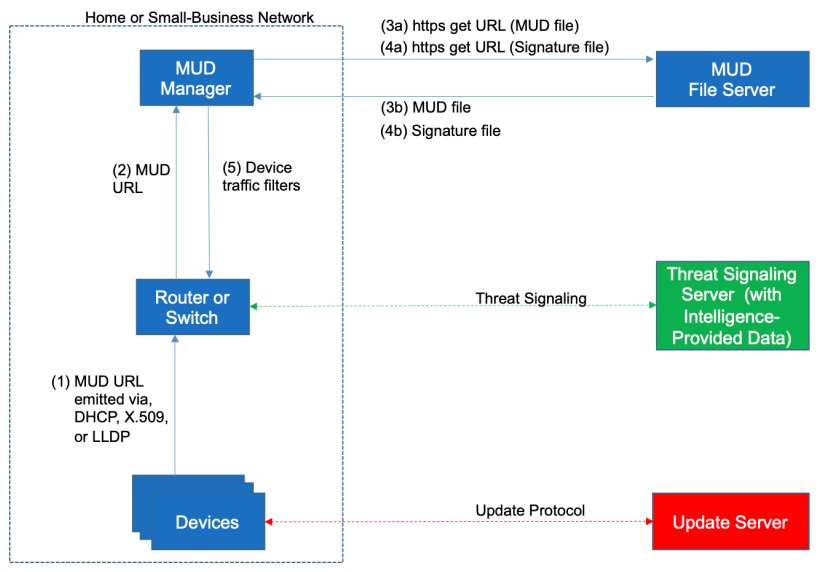
\includegraphics[width=0.95\textwidth]{figures/nist-mud-arch.png}
	\end{center}
	\caption{NIST MUD Reference Architecture}
	\label{fig:NIST MUD Reference Architecture}
\end{figure}
% section Manufacture Usage Description (end)

\section{Physical Unclonable Function} % (fold)
\label{sec:Physical Unclonable Function}

% TODO: (aver) add difference to 'physically unclonable function'

In order to be able to track IoT nodes in a blockchain, they need to be uniquely identifiable, in our case even in a
distributed manner, using e.g., Distributed Identifiers, DIDs.
Common practices are based on placing a cryptographic key into a nonvolatile electrically erasable programmable
read-only memory (EEPROM) or battery-backed static random-access memory (SRAM) and use hardware cryptographic operations
such as digital signatures or encryption, which is all expensive in design and power consumption. \cite{herder2014physical}

PUFs are unpredictable and uncontrollable, therefore making it unclonable and an ideal security vector. They are
dependent on random physical factors introduced during manufacturing, e.g., inequalities of SRAM cells, although factors
such as the altering of the physical components, voltage and temperature need to be taken into account. \cite{vinagrero2023sram}
For reasons of simplicity and because it is not the main focus of this thesis, we will neglect this aspect.
% TODO: Specify assumptions in another paragraph

By implementing the Challenge-Response Pair, CRP, is used to evaluate the microstructure, whereas a physical challenge
makes the device react, the response, in an unpredictable, but repeatable way.
In order to turn this 'silicon key' into a cryptographic root key, processing algorithms need to be applied, that ensure
that the distribution of 0s and 1s are uniform. \cite{herder2014physical}

\subsection{SRAM-Based PUF Readouts} % (fold)
\label{sec:SRAM-Based PUF Readouts}

Methods of creating identifiers that are unique to devices exist, such as SRAM-Based Physical Unclonable Function, PUF,
readouts. Therein PUFs are among the most cost-effective security primitives to establish hardware trust.
\cite{holcomb2007initial}

Even though the evaluation process of the characterization of guarantee over lifetime and differing operating conditions
are still subject to research following metrics have become widespread: \textit{reliability}, the variation of bit-wise
startup patterns; \textit{uniformity}, i.e., the repeatability and reproducibility on a given device after any amount of
restarts; \textit{uniqueness}, the probability of other devices with same signatures; \textit{bit-aliasing}, the
probability of specific bit position of the signature to be biased towards 0 or 1. \cite{vinagrero2023sram}
% subsection SRAM-Based PUF Readouts (end)

% TODO: (aver) challenges, vulnerabilities

% section Physical Unclonable Function (end)
\section{Over the Air IoT updating} % (fold)
\label{sec:Over the Air  IoT updating}
In order to stray away from the classic client-server architecture for updating devices, which demonstrate a single
point of failure, we will discuss other decentralized methods to achieve Over the Air, OTA, updates for IoT devices.

\subsection{Distributed OTA} % (fold)
\label{sub:Distributed OTA}
\textbf{\textit{TODO}}
% subsection Distributed OTA (end)
% section Over the Air IoT updating (end)

\section{Networking} % (fold)
\label{sec:Networking}
\textbf{\textit{TODO}}
\subsection{Software-Defined Networking} % (fold)
\label{sub:Software-Defined Networking}
\textbf{\textit{TODO}}
% subsection Software-Defined Networking (end)

\subsection{Network Functions Virtualization} % (fold)
\label{sub:Network Functions Virtualization}
\textbf{\textit{TODO}}
% subsection Network Functions Virtualization (end)
% section Networking (end)

\chapter{Related Work}

% NOTE: compares, contrasts, synthesizes, and provides introspection about the available knowledge for
% a given topic or field

\section{CERTIFY}
\section{CERTIFY} % (fold)
\label{sec:CERTIFY}

This thesis is carried out in conjunction with the CERTIFY project.

The National Institute for Standard and Technology has a few ongoing projects and white papers on security related
mitigation methods for IoT devices.

% section CERTIFY (end)


\section{DLT-based Asset-Tracking} % (fold)
\label{sec:DLT-based Asset-Tracking}

Neisse et al. (2017) analyzed how blockchain-based approaches might be used for data accountability and provenance
tracking under the then recently released GDPR legislation, highlighting challenges of scalability and considering
sharding as a method to address it. \cite{neisse2017blockchain} Further they also mentioned issues of clonability of
the tracked assets, which we can also correlate to the physical assets that are tracked inside blockchain.

% section DLT-based Asset-Tracking (end)


\section{Cybersecurity of IoT Devices} % (fold)
\label{sec:Cybersecurity of IoT Devices}


In order to maintain participation rights for only valid users/clients, Manufacturer Usage Descriptions, MUDs, are
getting more and more relevant, as also the National Institute for Standards and Technology, NIST, have been considering
their use cases. \cite{dodson2021securing}


\subsection{SRAM-based PUF Readouts} % (fold)
\label{sub:SRAM-based PUF Readouts}

We will also be considering using SRAM-based PUF readouts in our device configurations in order to get DIDs that are
absolutely unique for each device.

\cite{vinagrero2023sram}

% subsection SRAM-based PUF Readouts (end)

\subsection{Device Fingerprinting} % (fold)
\label{sub:Device Fingerprinting}

For classification of device capabilities NIST has been considering the usage of MUDs, so that devices do not step out
the bounds of their official and appointed capabilities. \cite{dodson2021securing}

% subsection Device Fingerprinting (end)
% section Cybersecurity of IoT Devices (end)

\chapter{Architecture and Design}
\label{chap:Architecture and Design}
% Apparently one needs to explain the architecture in this part. No mention of tools and co.

\begin{figure}
	\begin{center}
		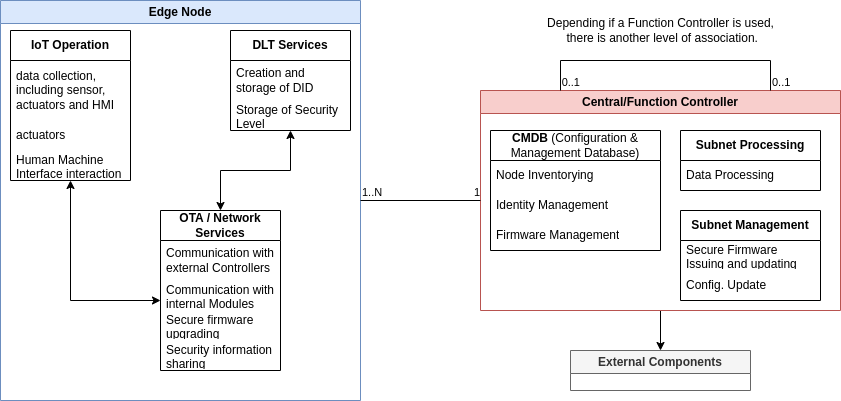
\includegraphics[width=0.95\textwidth]{figures/device-architecture-overview.png}
	\end{center}
	\caption{Device Architecture Overview}
	\label{fig:device-architecture-overview}
\end{figure}

\section{Actors} % (fold)
\label{sec:Actors-design}
In our architecture there will be a few actors, that play various roles, outlined in the below sections.

There will be a summarized device entity, that will be split up into two devices, as seen below in
Section~\ref{sec:Physical Components}, and further explained in Chapter~\ref{chap:Use Case Definition - Connected Cabin
	System}.
There will be a Manufacturer, that is responsible for the fabrication of said devices, as well as the creation of
Certificates and credentials, that will later be used by the devices and other entities for verification.
Further there shall be an auditor, that inspects said credentials and verifies them, or the necessary cases also
invalidation.
Finally an entity Infrastructure shall exist, that will enable the communication facilities for the entities.

We will assume a simplified and already predefined \textit{Authentication, Authorization and Accounting}, AAA, server
in order to simplify our environment.

Further external stakeholders include a certification authority and a vulnerability database.
% section Actors (end)

\section{Physical Components} % (fold)
\label{sec:Physical Components}

The composition of our physical architecture will entail two main devices of importance for us, as later defined in more
detail in Chapter \ref{chap:Use Case Definition - Connected Cabin System}, Section~\ref{sec:System Components}.

% The edge and controller nodes fulfill different responsibilities.

\subsection{Edge Nodes} % (fold)
\label{sec:Edge Nodes}
The edge nodes, also Internet of Things, IoT, nodes, are the frontier where direct interaction happens, be that sensing,
actuating or interaction through a Human Machine Interface, HMI.

Each edge node is uniquely identifiable through a Decentralized Identifier, DID, which will later be used for device
verification for outside entities through usage of a DLT. Furthermore, security levels, access levels will be stored on
each device. Through the use of MUDs, each device will be defined to have certain capabilities and access privileges,
which all will be enforced by the controller node.

\textbf{\textit{Warning:}} Whether we will store our DID in a Secure Element, SE, or on the SoC FLASH, is not yet decided.
% subsection Edge Nodes (end)

\subsection{Controller Nodes} % (fold)
\label{sub:Controller Nodes}
The controller nodes are managers of the edge nodes. They fulfill various responsibilities and shield edge nodes in a
subnet for increased security control
% subsection Controller Nodes (end)

% section Physical Components (end)

\section{Onboarding} % (fold)

\label{sec:Onboarding}
\begin{figure}
	\begin{center}
		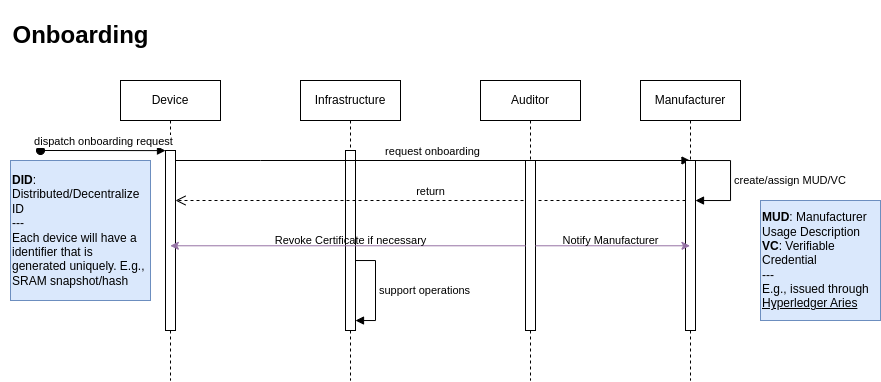
\includegraphics[width=0.95\textwidth]{figures/onboarding-sequence-diagram.png}
	\end{center}
	\caption{Onboarding Sequence Diagram}
	\label{fig:onboarding-sequence-diagram}
\end{figure}

The onboarding of a device can be observed in a sequence diagram in Figure~\ref{fig:onboarding-sequence-diagram}.
All of the actors in Section~\ref{sec:Actors-design} are involved.

We assume a device has been manufactured and that it is now at the desired location. In the first time setup, the device
will be either programmed to create a DID on setup, or will be assigned/created one in the manufacturing process,
depending on the computational and hardware facilities. Both an edge and controller node shall have their DID, since
both will be managed and or inventoried by another instance or entity.
Necessary for this process is a valid MUD file, also issued by the manufacturer, on device fabrication or on first time
setup. This MUD does not necessarily need to be on the device, but a URL is needed, which points to the location of such
file, see Section~\ref{sec:Manufacture Usage Description}.
Each device shall request and onboarding by the manufacturer, which then verifies the DID, and in case of validity
issues a Verifiable Credential, VC, to the device.

In more detail, an edge node shall request onboarding from the controller node, which then forwards the request to the
manufacturer.

The Auditor then proceeds to verify the validity of the VC and checks for any known vulnerabilities, that might be
affect the device that requested the VC. The Auditor shall also monitor the VC periodically, in order to check for any
vulnerabilities the devices themselves might have missed. In case of an insecurity or vulnerability the auditor shall
notify both the device and the manufacturer and revoke the VC, until the device has been known to update its Firmware to
a secure version, see Section~\ref{sec:Secure Firmware Updating}.

\subsection{VC Verification} % (fold)
\label{sub:VC Verification}
The verification of a VC may happen through the usage of a Smart Contract. Therein the invalidation of
said smart contract happens through the fulfillment of the contract condition, which could be a discovered
vulnerability.
% subsection VC Verification (end)

% section Onboarding (end)


% NOTE: (aver) Emphasis 1
\section{Inventorying} % (fold)
\label{sec:Inventorying}

\begin{figure}
	\begin{center}
		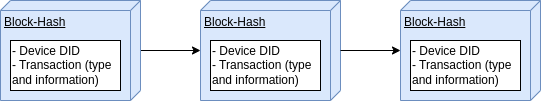
\includegraphics[width=0.95\textwidth]{figures/dlt-architecture.png}
	\end{center}
	\caption{DLT Architecture}
	\label{fig:dlt-architecture}
\end{figure}

Getting to the first emphasis of our thesis, we will explore, how we can safely and efficiently store and keep an
inventory of our devices.

For this we will rely on a DLT, in which any action will be saved as a block. The DLT used shall be permissioned and
possibly private, so that only those permissioned may be a part of this blockchain.
The DLT will work as a decentralized Configuration and Management Database, CMDB, as seen in
Figure~\ref{fig:dlt-architecture}. Transaction will be fulfilled by the controller node as indicated in
Figure~\ref{fig:device-architecture-overview}.

% section Inventorying (end)


\section{Operations} % (fold)
\label{sec:Operations}

In order to be able to simulate the whole device lifecycle, we will also implement simple day-2-day operations, such as
reading out sensors, actuating or minor interactions through HMIs.

Depending on the device type, edge or controller, further responsibilities are expected. A controller node has to
constantly check against the DLT, whether there were any new vulnerabilities discovered and if the VC was consequently
revoked, as mentioned before, the controller node has to check its own status, as well as the ones of the subnet of
edge nodes. If such were the cases, concerned devices need be recertified.

% TODO: (aver) possibly extend with real-time local security monitoring

% section Operations (end)


% NOTE: (aver) Emphasis 2
\section{Secure Firmware Updating} % (fold)
\label{sec:Secure Firmware Updating}

As the second emphasis of this thesis we aim to provide a secure update mechanism for outdated and or vulnerable
firmware versions.

\begin{figure}
	\begin{center}
		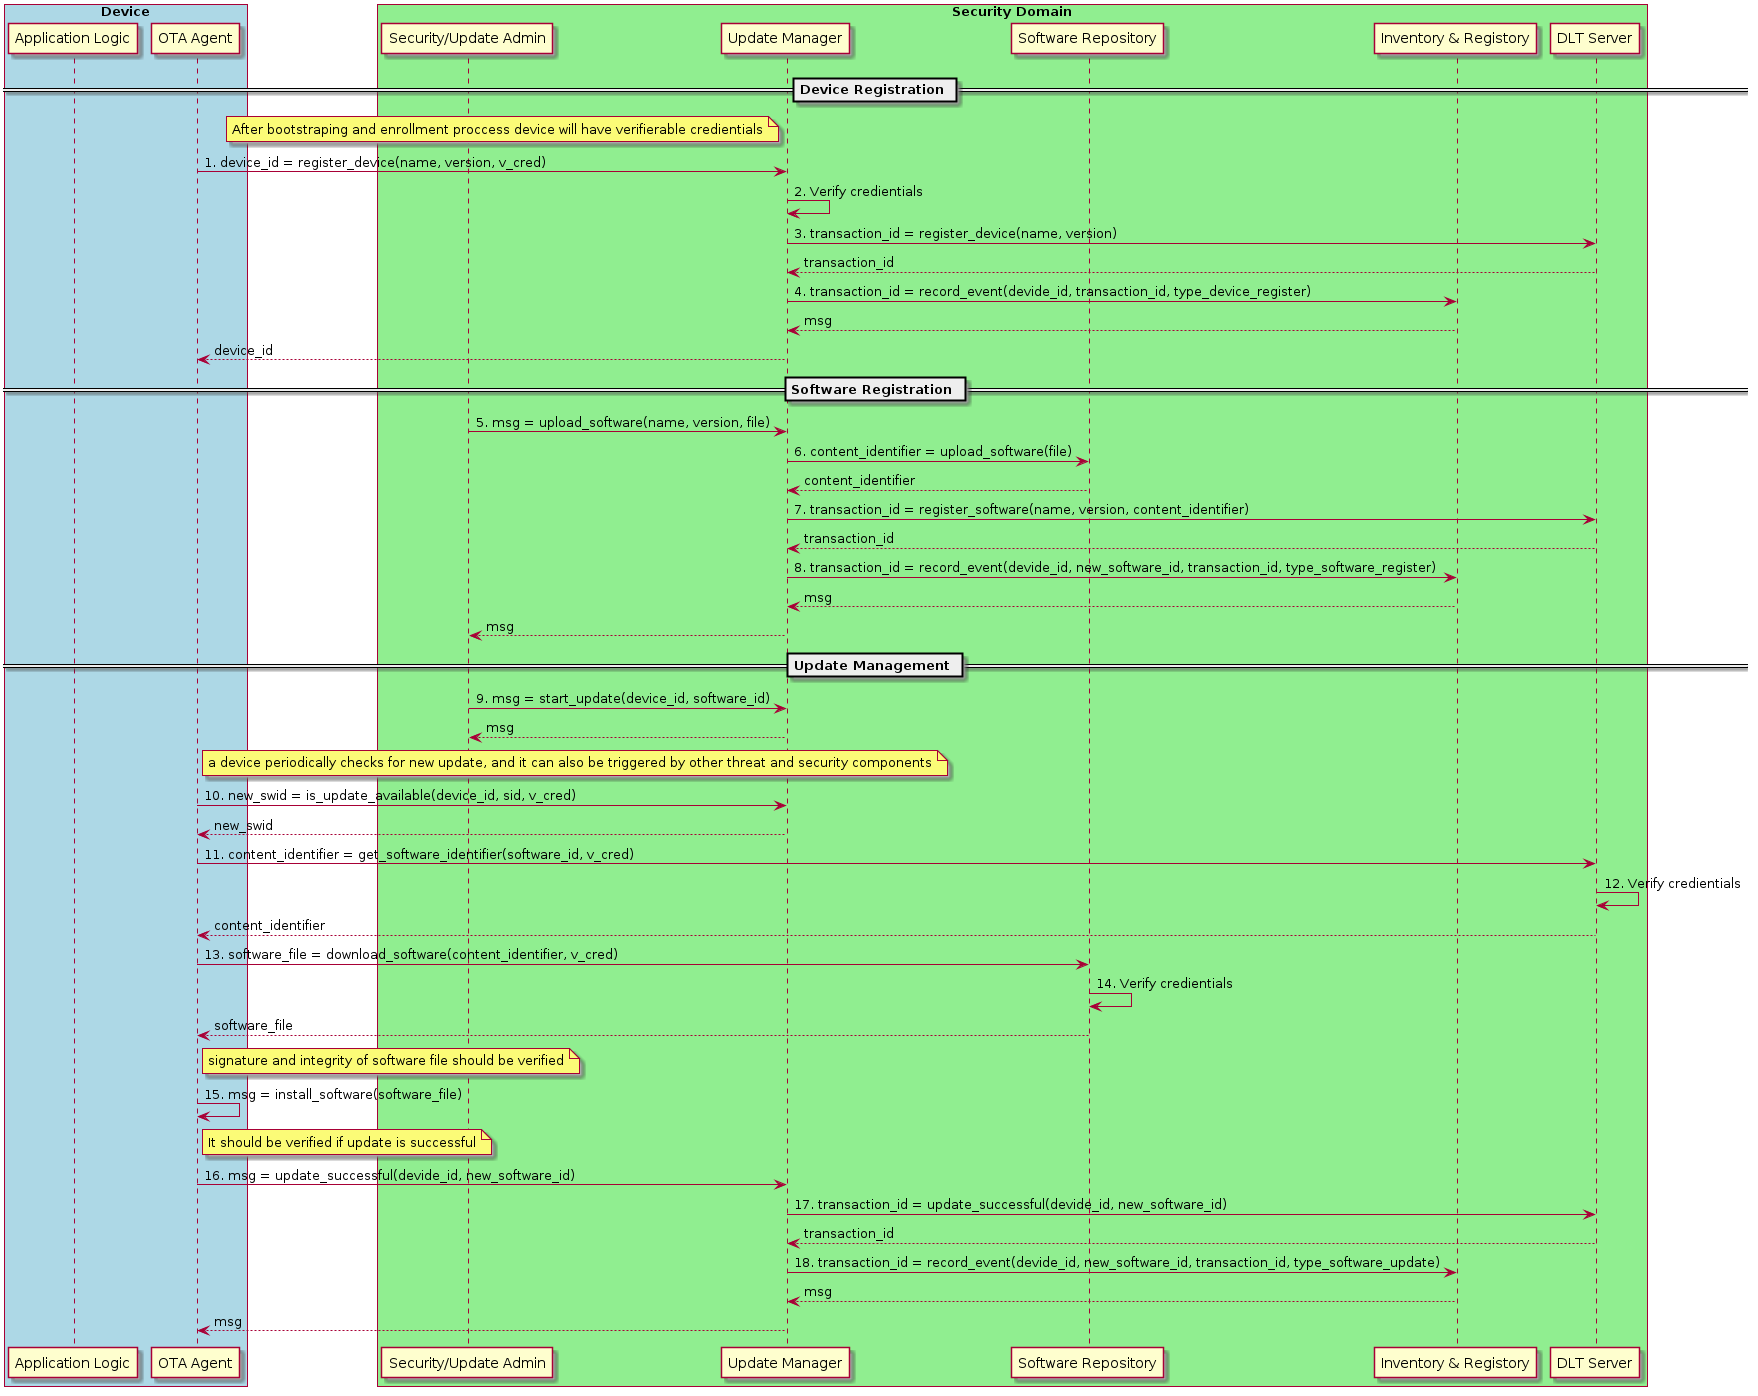
\includegraphics[width=0.95\textwidth]{figures/ota-update-certify-V1.2.png}
	\end{center}
	\caption{CERTIFY OTA Update \cite{certifyproject2023}}
	\label{fig:ota-update-certify}
\end{figure}

% TODO: (aver) research and explain possible update mechanisms.

% section Secure Firmware Updating (end)

\section{Secure Information Sharing} % (fold)
\label{sec:Secure Information Sharing}

In order to enable the sharing of information related to the security of the device, we will rely on directional
information sharing, meaning, the devies receive vulnerability information, updates and MUD files, while external
sources receive status updates and co. of the devices concerned.

These information can be embedded into transaction inside the DLT, depending on the importance of the information, it
can also be shared through less sophisticated measures.

% section Secure Information-Sharing (end)

\chapter{Use Case Definition - Connected Cabin System}
\label{chap:Use Case Definition - Connected Cabin System}

\begin{figure}
	\begin{center}
		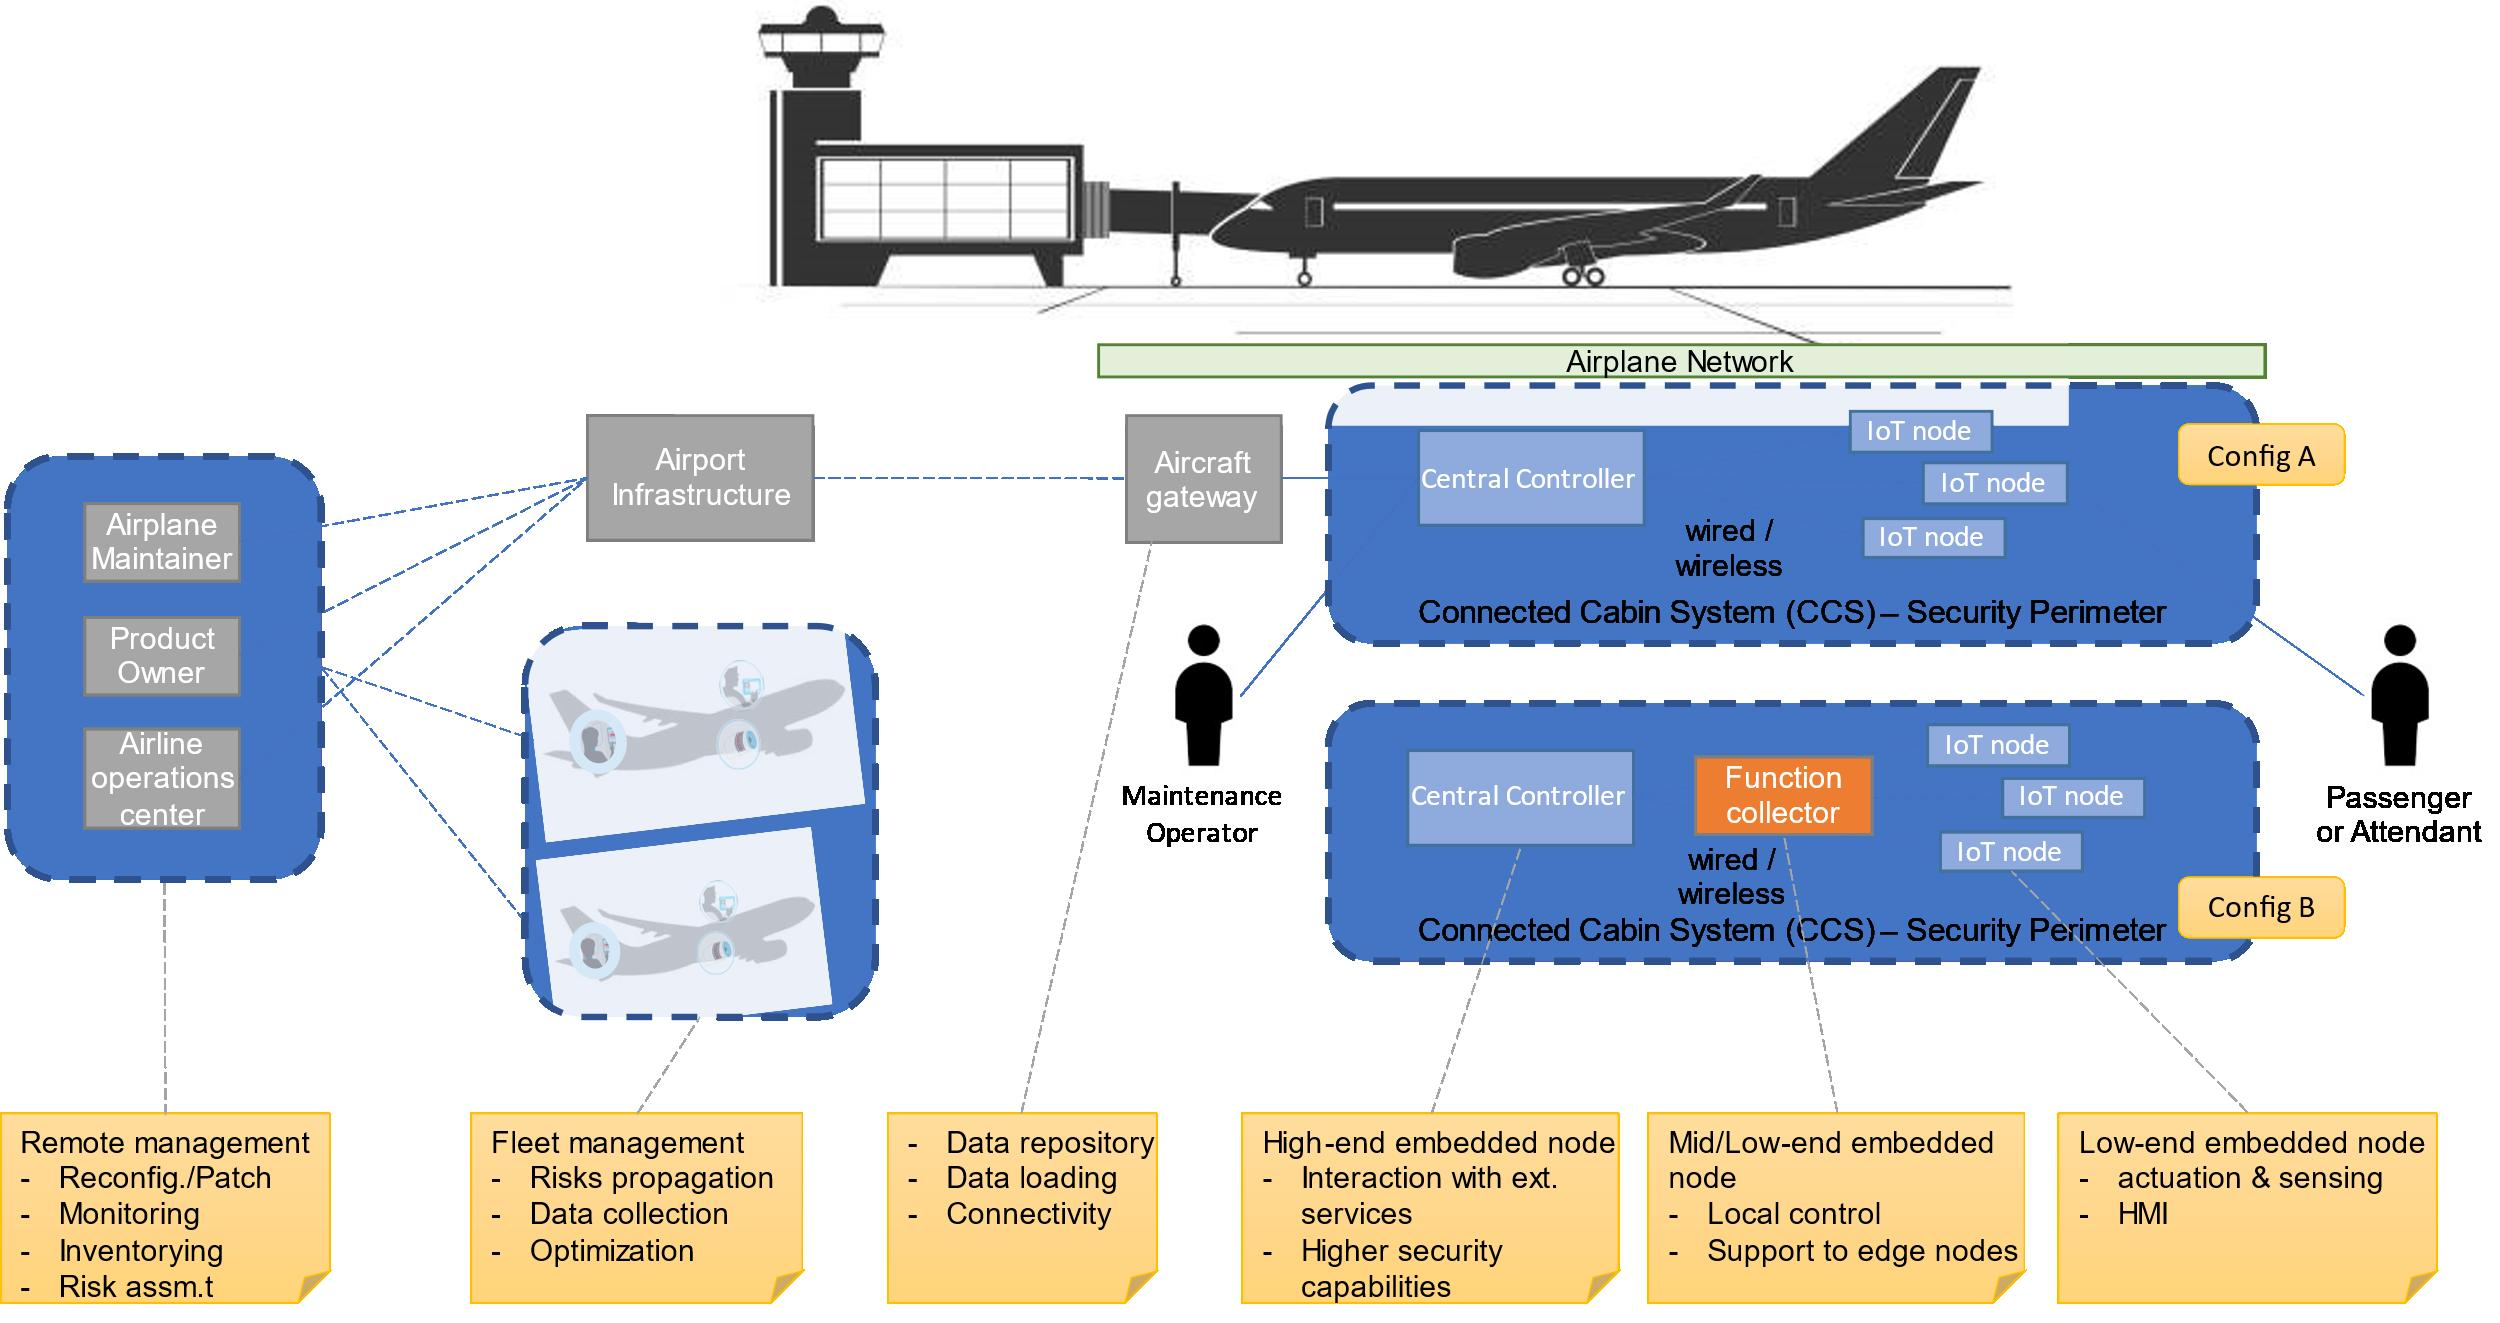
\includegraphics[width=0.95\textwidth]{figures/collins-ccs.jpg}
	\end{center}
	\caption{Collins CCS}
	\label{fig:Collins CCS}
\end{figure}

\section{Background} % (fold)
\label{sec:Background}

Our use case will take the CCS scenario from Figure~\ref{fig:Collins CCS} into consideration and build up on their use
cases, which were borrowed from the CERTIFY project \cite{certifyproject2023}.

Nowadays more and more IoT devices are being deployed to aircraft cabins to improve passenger experience and airline
operations. Benefits span from remote PHM to reduced maintenance time, while also supporting a
continuous (re)certification process. % TODO: (aver) add source, maybe from certify

% section Background (end)

\section{Actors} % (fold)
\label{sec:Actors}

We will consider following actors for our use case.

\begin{itemize}
	\item Airline:
	      Owns the aircraft and oversees daily interactions and systems operations.
	\item Airplane maintainer: They could be e.g., the airplane manufacturer. Oversees maintenance of the aircraft,
	      including the integration of systems designed by different manufacturers and their configuration.
	\item Product Owner: Oversees design and maintenance of systems deployed in the aircraft on assignment of the
	      airplane maintainer.
	\item Maintenance operator: They work for the airplane maintainer. Their responsibilities include e.g.,
	      the replacement of devices or on-site software upgrades of e.g., portable data loaders.
	\item Passenger, Attendant, Pilot: They interact with the aircraft through sensors, actuators or HMI.
\end{itemize}

% section Actors (end)

\section{System Components} % (fold)
\label{sec:System Components}

We will consider an aircraft to have multiple networks, covering various aspects.
\begin{itemize}
	\item In-flight entertainment system
	\item Aircraft System
	\item Flight Maintenance
\end{itemize}

For our use case we will assume config 'A' as the main configuration of the networks, where edge nodes are connected to
a central controller that manages the edge nodes as a subnet.
\begin{itemize}
	\item IoT / Edge Nodes: low-end devices, including actuation, sensing or HMI capabilities, with limited
	      room for hardware and software based cybersecurity, that requires offloading to a more capable
	      instance.
	\item Central Controller: High-end devices with ability to host full-fledged security functionalities.
\end{itemize}

External communication will take place through aircraft gateway offering services for data repository, data loading and
connectivity with external environment. The airline operations center, product owner and airplane maintainer can interact
through the airport infrastructure. A technician may directly access the aircraft if necessary.

% section System Components (end)


\section{Scenarios} % (fold)
\label{sec:Scenarios}

\subsection{Installation of Connected Cabin Systems} % (fold)
\label{sub:Installation of Connected Cabin Systems}

\begin{table}
	\caption{Actors involved}
	\label{tab:Actors involved installation}
	\begin{center}
		\begin{tabular}{ |p{2.5cm}|p{2.5cm}|p{2.5cm}|p{2.5cm}|p{2.5cm}| }
			\hline
			Airline & Airplane Maintainer & Product Owner & Maintenance Operator & Passenger, Attendant, Pilot \\
			\hline
			X       & X                   & X             & X                    & X                           \\
			\hline
		\end{tabular}
	\end{center}
\end{table}

\begin{table}
	\caption{Lifecycle stages involved}
	\label{tab:Lifecycle stages involved installation}
	\begin{center}
		\begin{tabular}{ |c|c|c|c|c| }
			\hline
			Bootstrapping & Operation & Update & Repurposing & Decommissioning \\
			\hline
			X             & -         & X      & -           & X               \\
			\hline
		\end{tabular}
	\end{center}
\end{table}


\subsubsection{Goals}

The goals of this scenario include bootstrapping and customization of devices for specific deployment, updating and
decommissioning of previous systems, guaranteeing a reset to a known and fresh, wiped data, state.
Table~\ref{tab:Actors involved installation} highlights the involved actors and
Table~\ref{tab:Lifecycle stages involved installation} shows the stages involved in this scenario.

\subsubsection{Pre-condition}

In order for this scenario to be valid, following pre-conditions need to be met:
\begin{itemize}
	\item Actors involved can establish a secure connection with the aircraft, wireless or wired, through airport
	      infrastructure
	\item Airport and Aircraft network infrastructure can receive authorization requests for needed connections from
	      the external environment.
	\item The Maintenance Operator is provided access to the airplane and to maintenance ports of the target CCS.

\end{itemize}

\subsubsection{Sub-Scenario 1: Component Installation}

\begin{figure}
	\begin{center}
		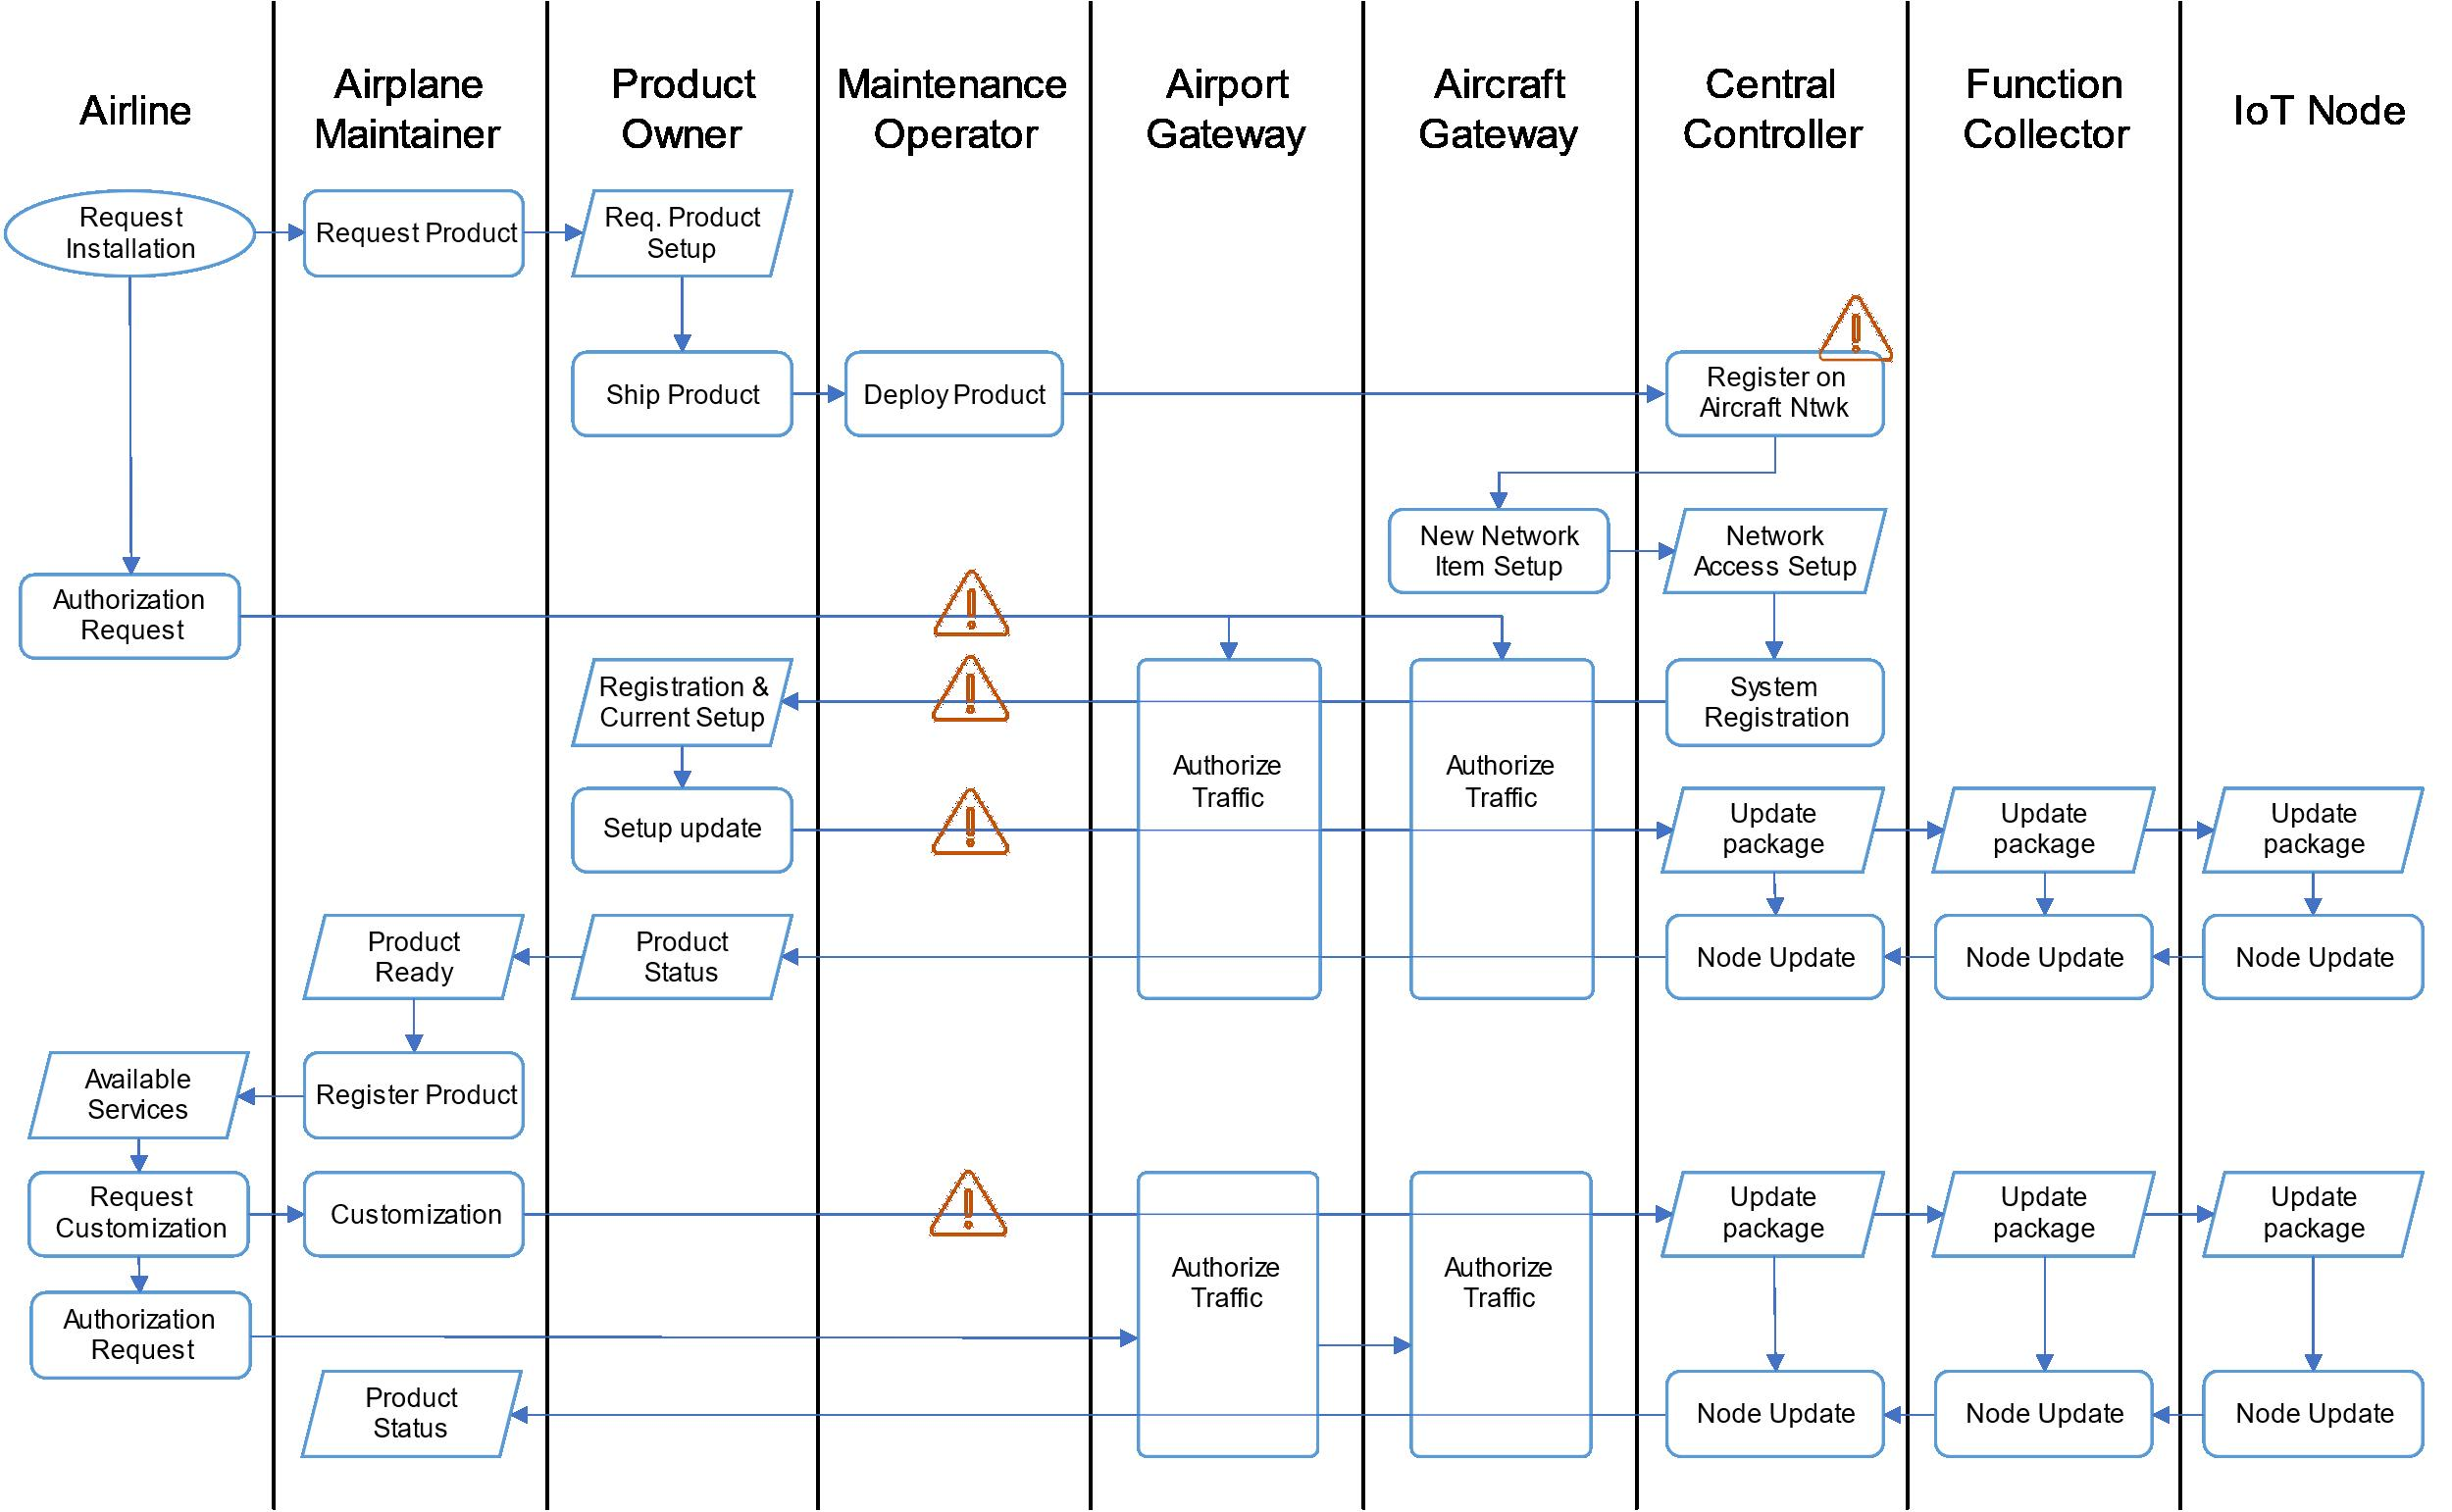
\includegraphics[width=0.95\textwidth]{figures/collins-s1-installation.jpg}
	\end{center}
	\caption{Collins Scenario 1: Device Installation}
	\label{fig:collins-s1-installation}
\end{figure}

\paragraph{Flow of Events}

The flow of events can be tracked in Figure~\ref{fig:collins-s1-installation} and is verbalized as follows:

\begin{itemize}
	\item Airline requests installation of new component to the Airplane Maintainer also issuing an authorization
	      request to Airport and Airplane gateways.
	\item The request is forwarded to the Product Owner and then to the Maintenance Operator, who oversees the
	      physical deployment of the product.
	\item Once connected, Central Controller registers on the Aircraft Network and receives required setup to
	      complete network access and system registration.
	\item Product Owner is now able to reach the CCS, push configuration and security updates to the Central
	      Controller, as well as the Function Collector and IoT nodes.
	\item After the update, the product is registered and the Airplane Maintainer can offer remote services to the
	      Airline.
	\item The Airline requests a customization of the CCS. It is performed by the Airplane Maintainer by pushing an
	      update package and/or modifying specific configurations as allowed by the Product Owner API for
	      Maintenance.
	\item The new product status is confirmed with a feedback message.
\end{itemize}

\subsubsection{Sub-Scenario 2: Component Replacement}

\begin{figure}
	\begin{center}
		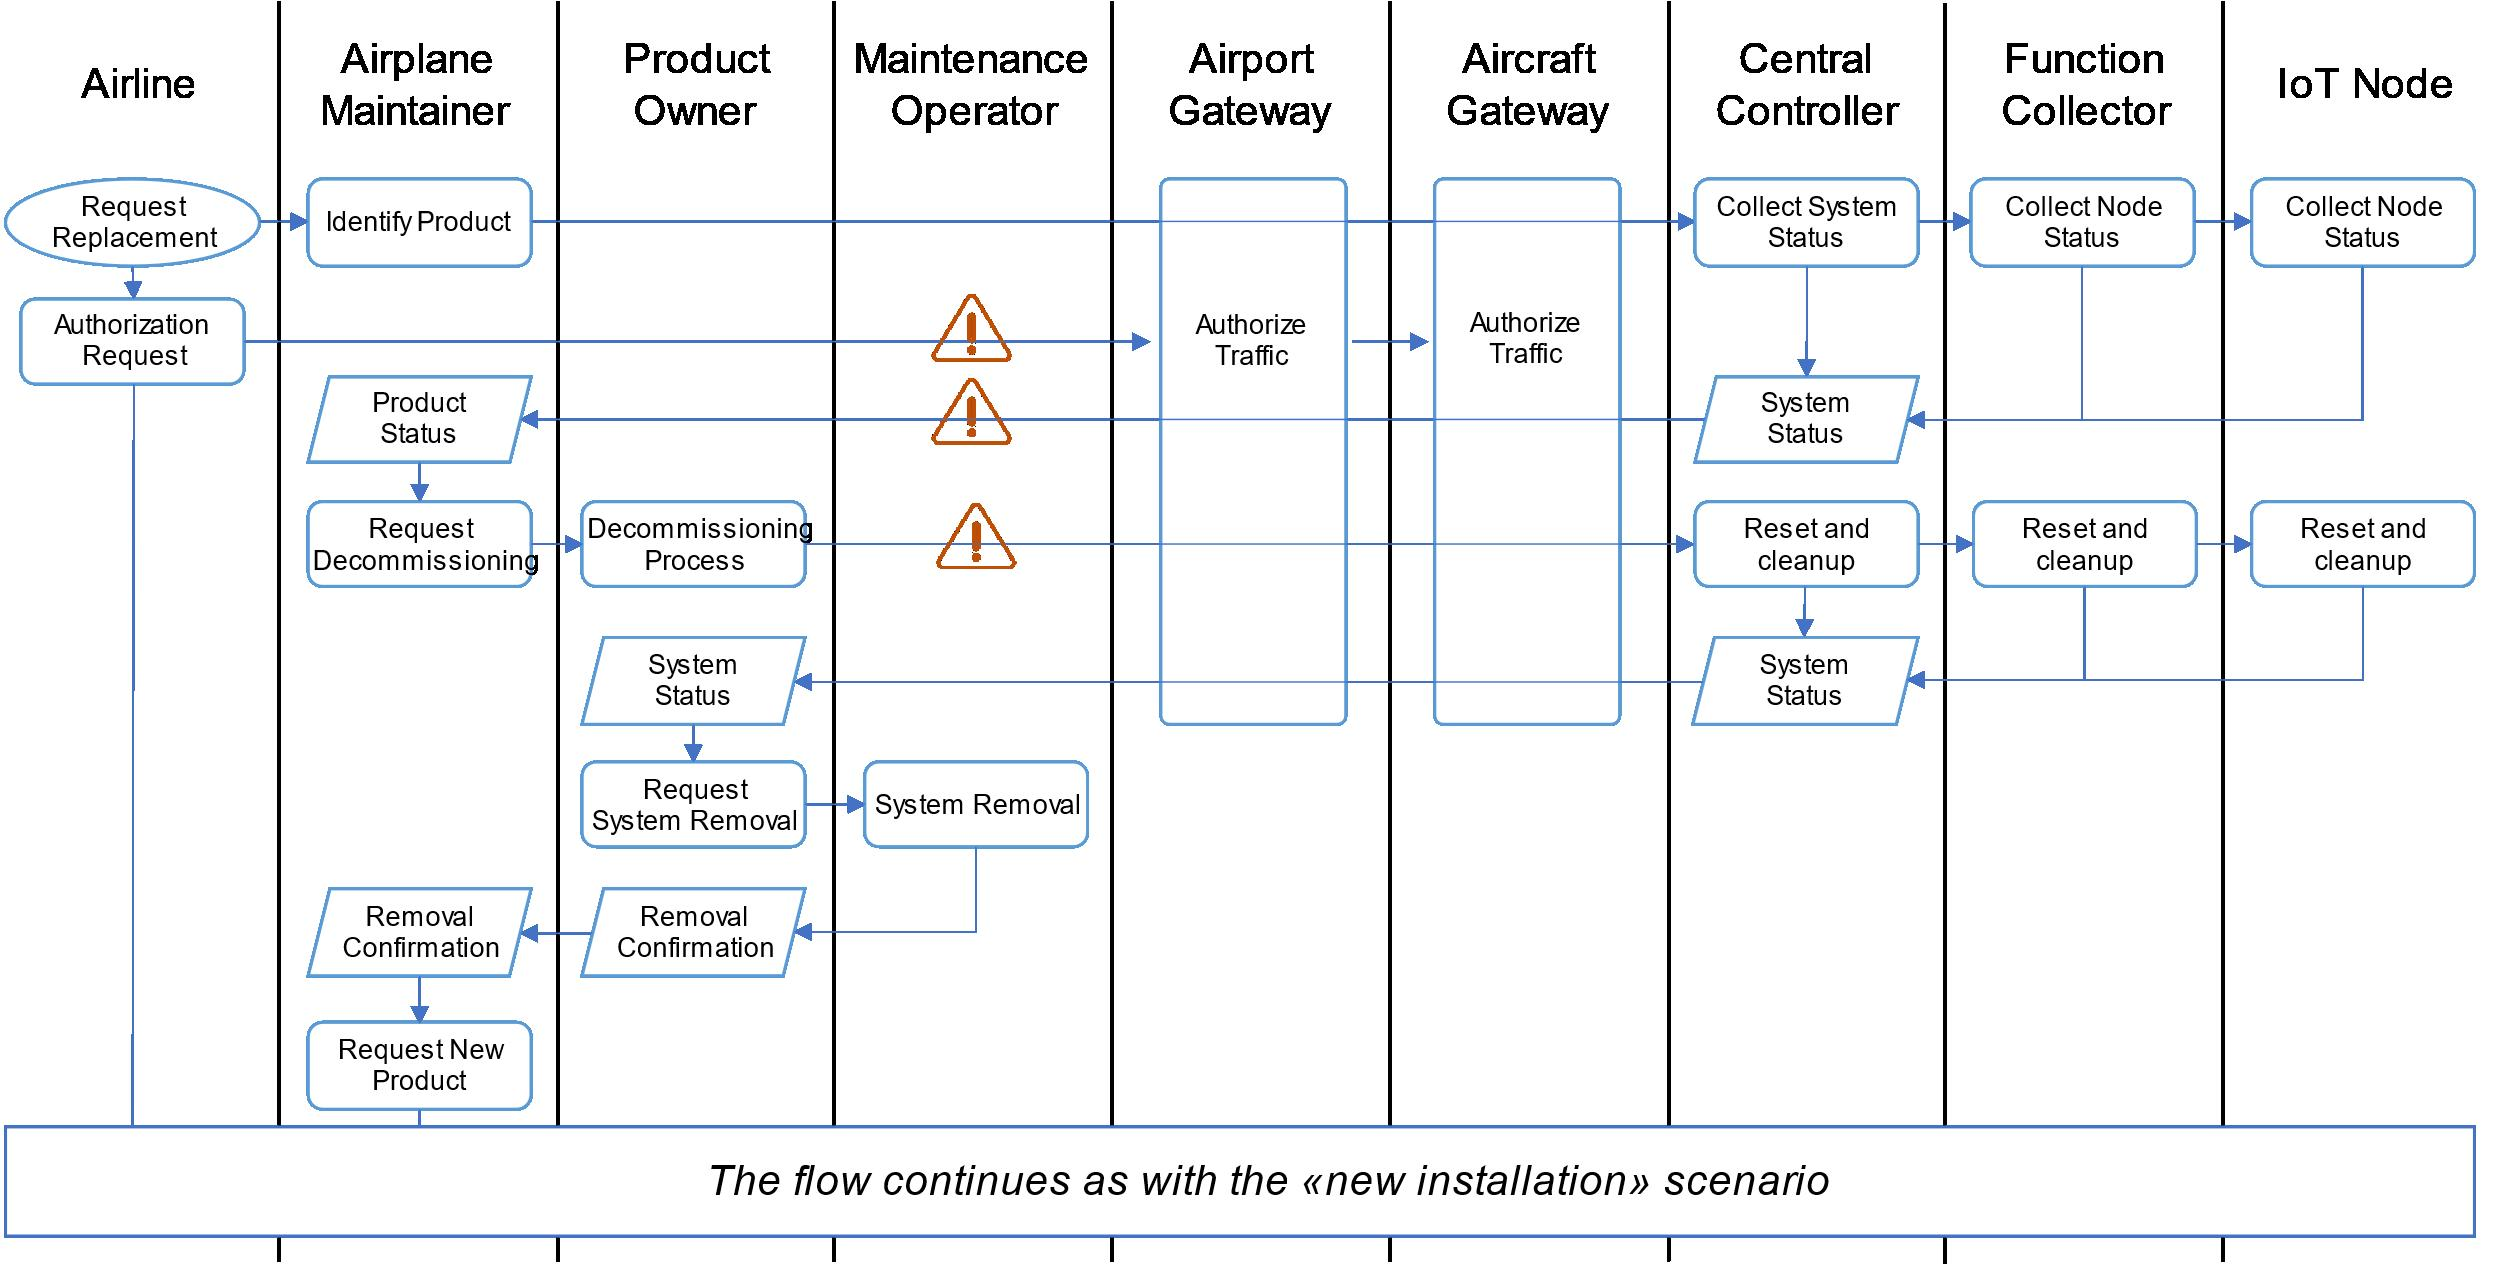
\includegraphics[width=0.95\textwidth]{figures/collins-s1-replacement.jpg}
	\end{center}
	\caption{Collins Scenario 1: Device Replacement}
	\label{fig:collins-s1-replacement}
\end{figure}

\paragraph{Flow of Events}

\begin{itemize}
	\item The Airline requests replacement of a component to the Airplane maintainer, also issuing an authorization
	      request to the Airport and Airplane Gateways.
	\item The Airplane Maintainer identifies the target product (location) and collects latest system status.
	\item The Airplane Maintainer issues a decommissioning request to the Product Owner and starts the
	      decommissioning process, which causes a reset and cleanup of all the nodes that will be replaced.
	\item After remote reset and clean-up, product owner requests the Maintenance Operator to physically remove the
	      system from the cabin.
	\item The product is then unregistered and can be dismissed.
	\item The remaining part continues with the 'New installation process flow'
\end{itemize}

\subsubsection{Post-Condition}

After completion of the Installation Scenario, following post-conditions need to be met:

\begin{itemize}
	\item New component is deployed in the CCS, integrated into the network, updated with latest security patches
	      and configured by the Airline for their specific needs.
	\item Component is securely onboarded in the CCS, unique identity and certificates are dispatched for
	      authentication.
	\item Regarding the configurations, their integrity is verified and confidentiality has been preserved.
\end{itemize}

\subsubsection{Attack Scenario}

As an alternative flow of events, i.e., in an attack scenario, highlighted by the yellow triangles in
Figure~\ref{fig:collins-s1-installation} and Figure~\ref{fig:collins-s1-replacement} following points were identified:

\begin{itemize}
	\item Attacker can inject malicious payloads in place of the intended one, (confidential) credentials provided
	      to the Central Controller for network access and authentication ca be stolen.
	\item IP sensitive data can be leaked by the Airplane Maintainer when retrieving the system status.
	\item The integrity of maintenance/reset/cleanup procedures can be compromised.
\end{itemize}

% subsection Installation of Connected Cabin Systems (end)

\subsection{System Operation and Monitoring} % (fold)
\label{sub:System Operation and Monitoring}

\begin{table}
	\caption{Actors involved operations}
	\label{tab:Actors involved}
	\begin{center}
		\begin{tabular}{ |p{2.5cm}|p{2.5cm}|p{2.5cm}|p{2.5cm}|p{2.5cm}| }
			\hline
			Airline & Airplane Maintainer & Product Owner & Maintenance Operator & Passenger, Attendant, Pilot \\
			\hline
			X       & X                   & X             & -                    & X                           \\
			\hline
		\end{tabular}
	\end{center}
\end{table}

\begin{table}
	\caption{Lifecycle stages involved}
	\label{tab:Lifecycle stages involved operations}
	\begin{center}
		\begin{tabular}{ |c|c|c|c|c| }
			\hline
			Bootstrapping & Operation & Update & Repurposing & Decommissioning \\
			\hline
			-             & X         & X      & -           & -               \\
			\hline
		\end{tabular}
	\end{center}
\end{table}

\subsubsection{Goals}

The goals of System Operations and Monitoring incorporate following points:

\begin{itemize}
	\item Periodic collection of data from airplane.
	\item Data offload/upload to ground stations for performance monitoring, optimization and PHM operations.
	\item Attendants interact with CCS through a HMI
	\item CCS Information is collected and stored in Gateway.
	\item A limited set of predefined reconfigurations may be performed on plane, when requested by Airline,
	      Maintainer or product owner.
\end{itemize}

\subsubsection{Pre-conditions}
\begin{itemize}
	\item Maintainers have established remote secure connection with the aircraft (wireless or wired) through the
	      airport infrastructure.
	\item Passengers/Attendants/Pilots can interact through HMI or are connected through other devices e.g., through
	      WiFi (possibly in the sense of bring you own device, BYOD).
	\item Device bootstrapping, enrollment, configuration, provisioning are completed for all devices, that are
	      (statically) part of the network.
	\item IoT devices are equipped with sensors to collect and store data that are then forwarded to their root
	      controller.
	\item Devices can securely store and transmit collected data.
\end{itemize}

\subsubsection{Flow of Events}

\ref{fig:collins-s2-data-collection-reconfig}
\ref{fig:collins-s2-data-unload-remote-analysis}
\ref{fig:collins-s2-data-load-remote-config}

\begin{itemize}
	\item IoT devices collect data during airplane operations, see Figure \ref{fig:collins-s2-data-collection-reconfig}
	\item Data is securely stored on-board, see Figure \ref{fig:collins-s2-data-collection-reconfig}
	\item Local computations over critical and non-critical data are executed in separate environments to reconfigure
	      the airplane/flight, see Figure \ref{fig:collins-s2-data-collection-reconfig}
	      \textbf{What is meant by this?}
	\item Remote entities are authenticated and a connection is established with the aircraft network through the
	      gateway, see Figure \ref{fig:collins-s2-data-load-remote-config}
	      \textbf{What Gateway? We are basically in flight so shouldn't we be disconnected? Otherwise this is
		      a scenario for Roaming}
	\item Data is downloaded from plane to ground
	\item In case of an Airplane fleet, Collective Analysis is performed, see Figure
	      \ref{fig:collins-s2-data-unload-remote-analysis}
	\item Upload new data and configurations, from ground to plane
	\item Data authenticity and integrity are verified before updating the configurations on the plane.
\end{itemize}

% \subsubsection{Sub-Scenario 1: Data Collection and Local Reconfiguration}
\begin{figure}
	\begin{center}
		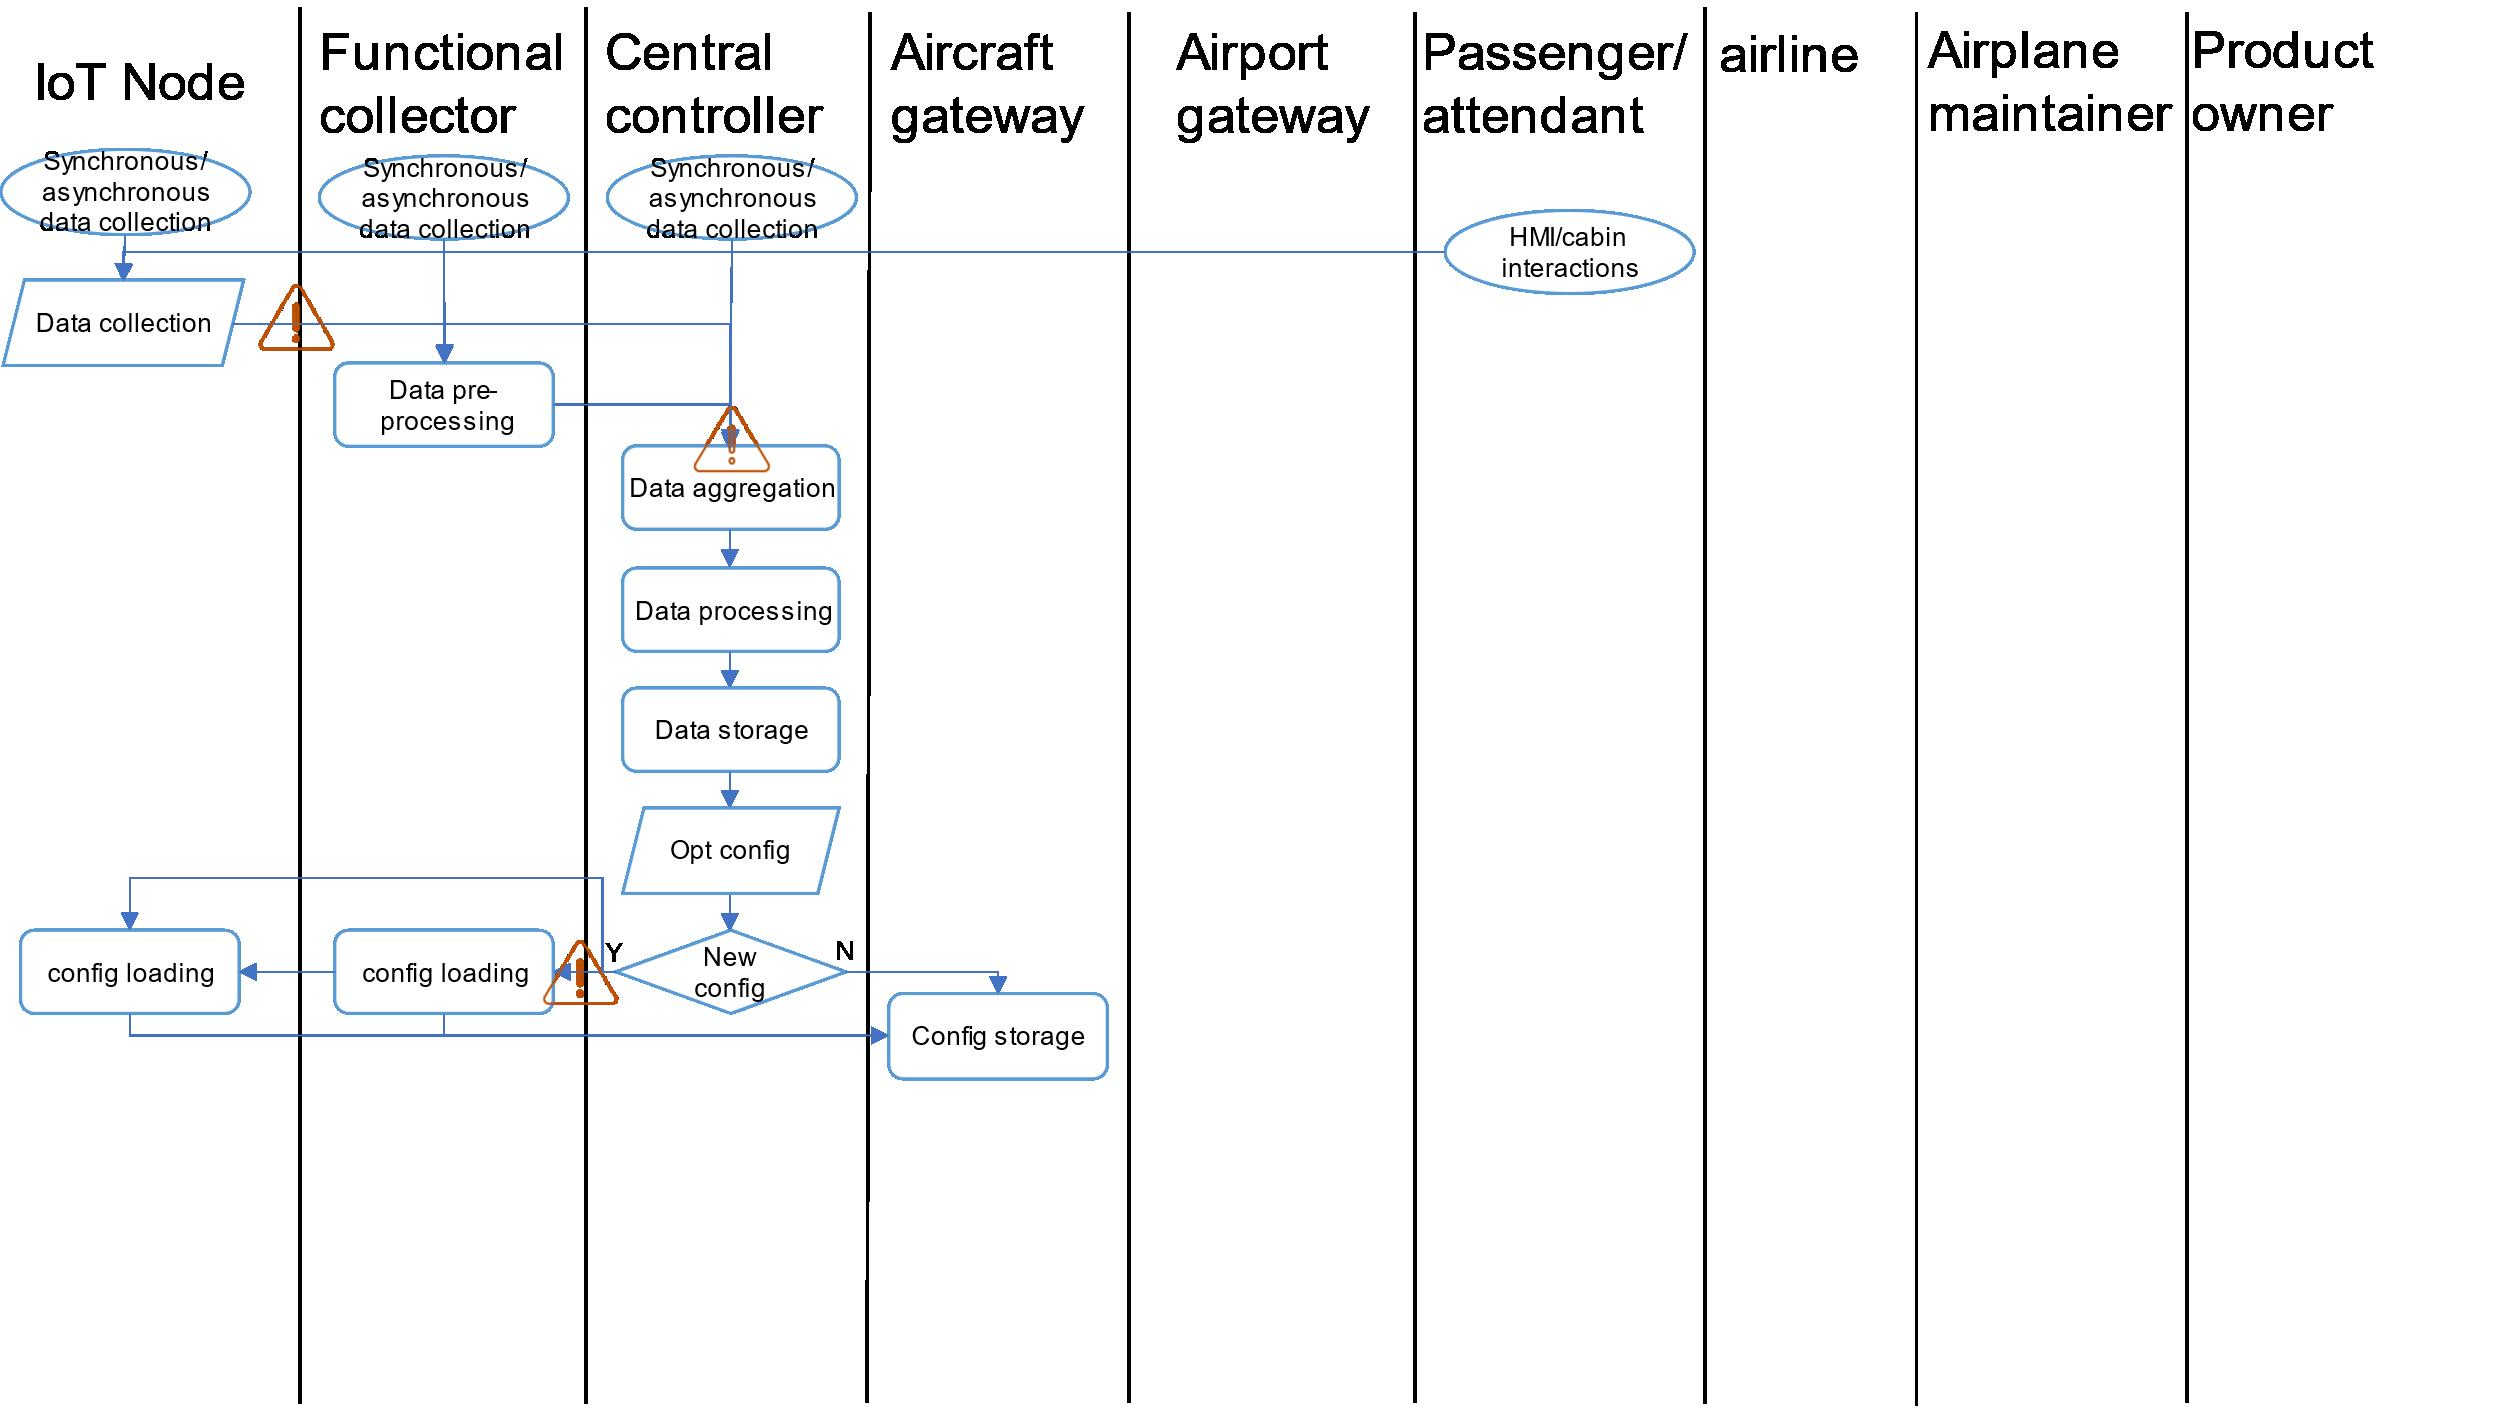
\includegraphics[width=0.95\textwidth]{figures/collins-s2-data-collection-reconfig.jpg}
	\end{center}
	\caption{Collins Scenario 2.1: Data Collection and Local Reconfiguration}
	\label{fig:collins-s2-data-collection-reconfig}
\end{figure}

% \subsubsection{Sub-Scenario 2: Data Unload and Remote Analysis}
\begin{figure}
	\begin{center}
		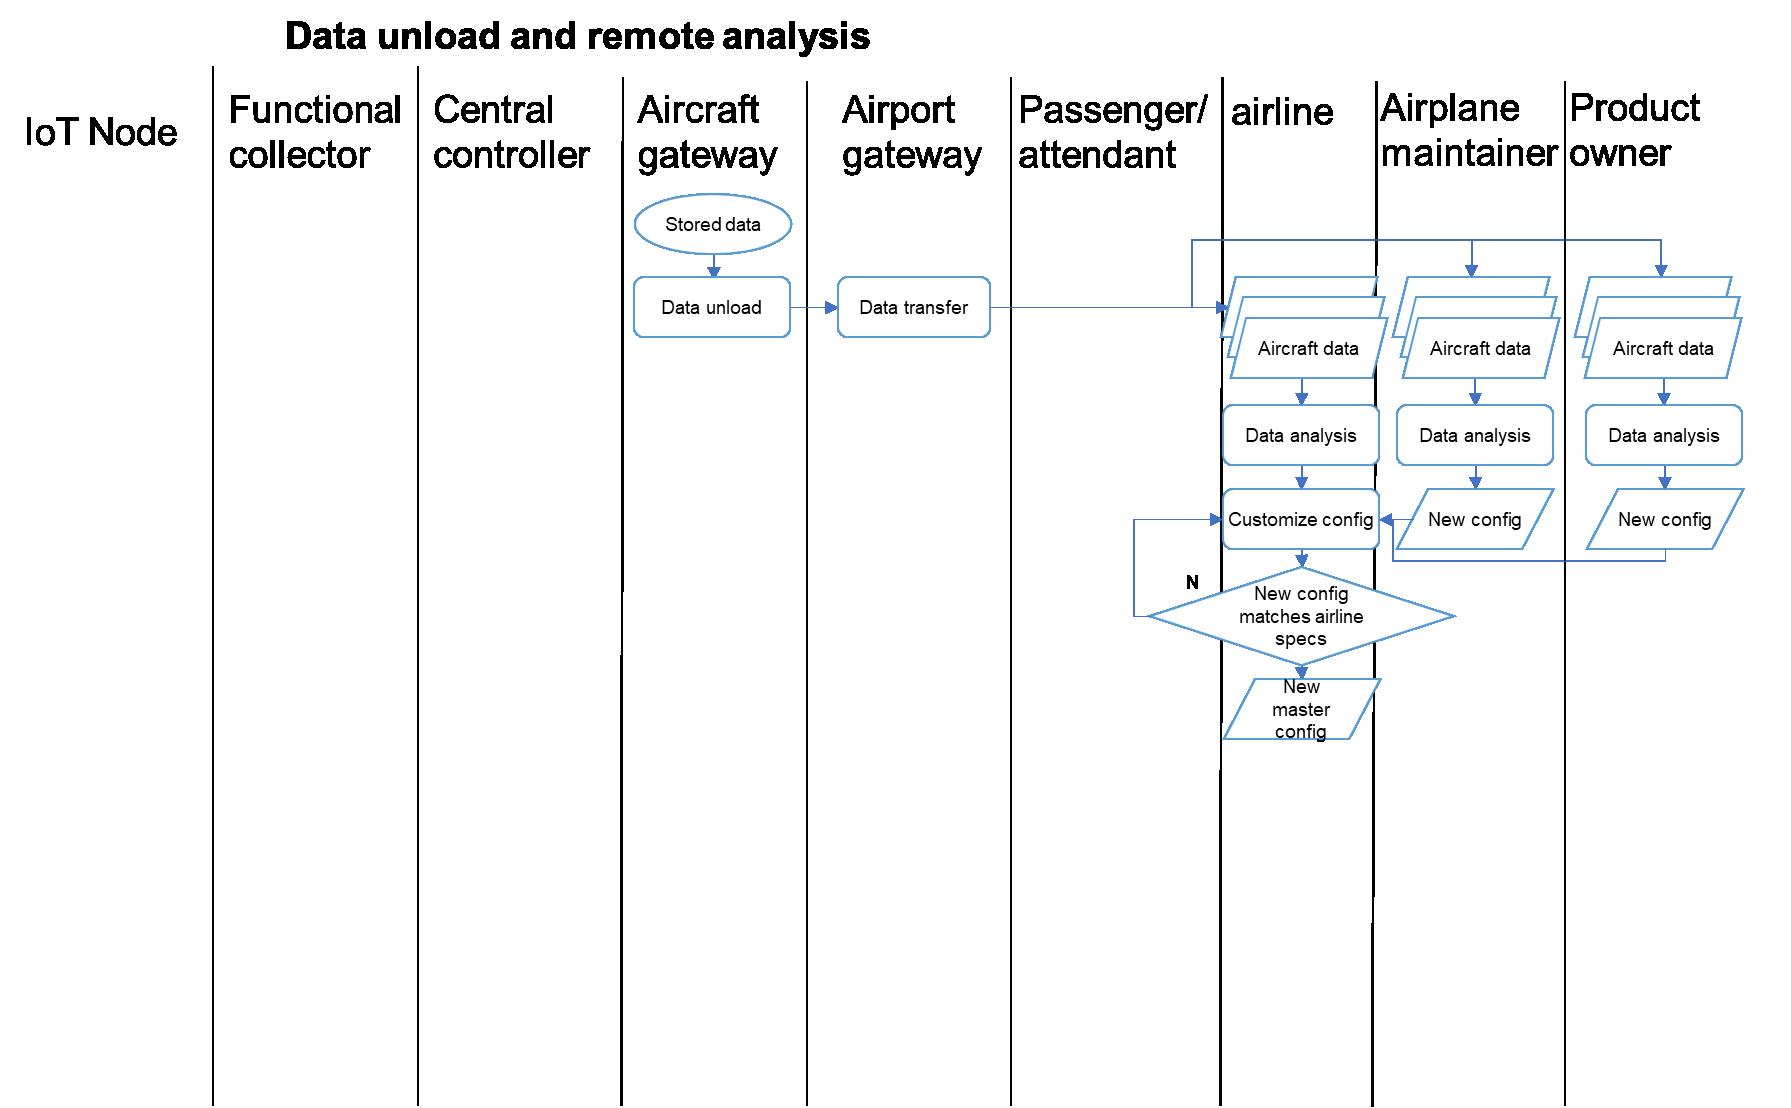
\includegraphics[width=0.95\textwidth]{figures/collins-s2-data-unload-remote-analysis.jpg}
	\end{center}
	\caption{Collins Scenario 2.2: Data Unload and Remote Analysis}
	\label{fig:collins-s2-data-unload-remote-analysis}
\end{figure}

% \subsubsection{Sub-Scenario 3: Data Load from Remote Config}
\begin{figure}
	\begin{center}
		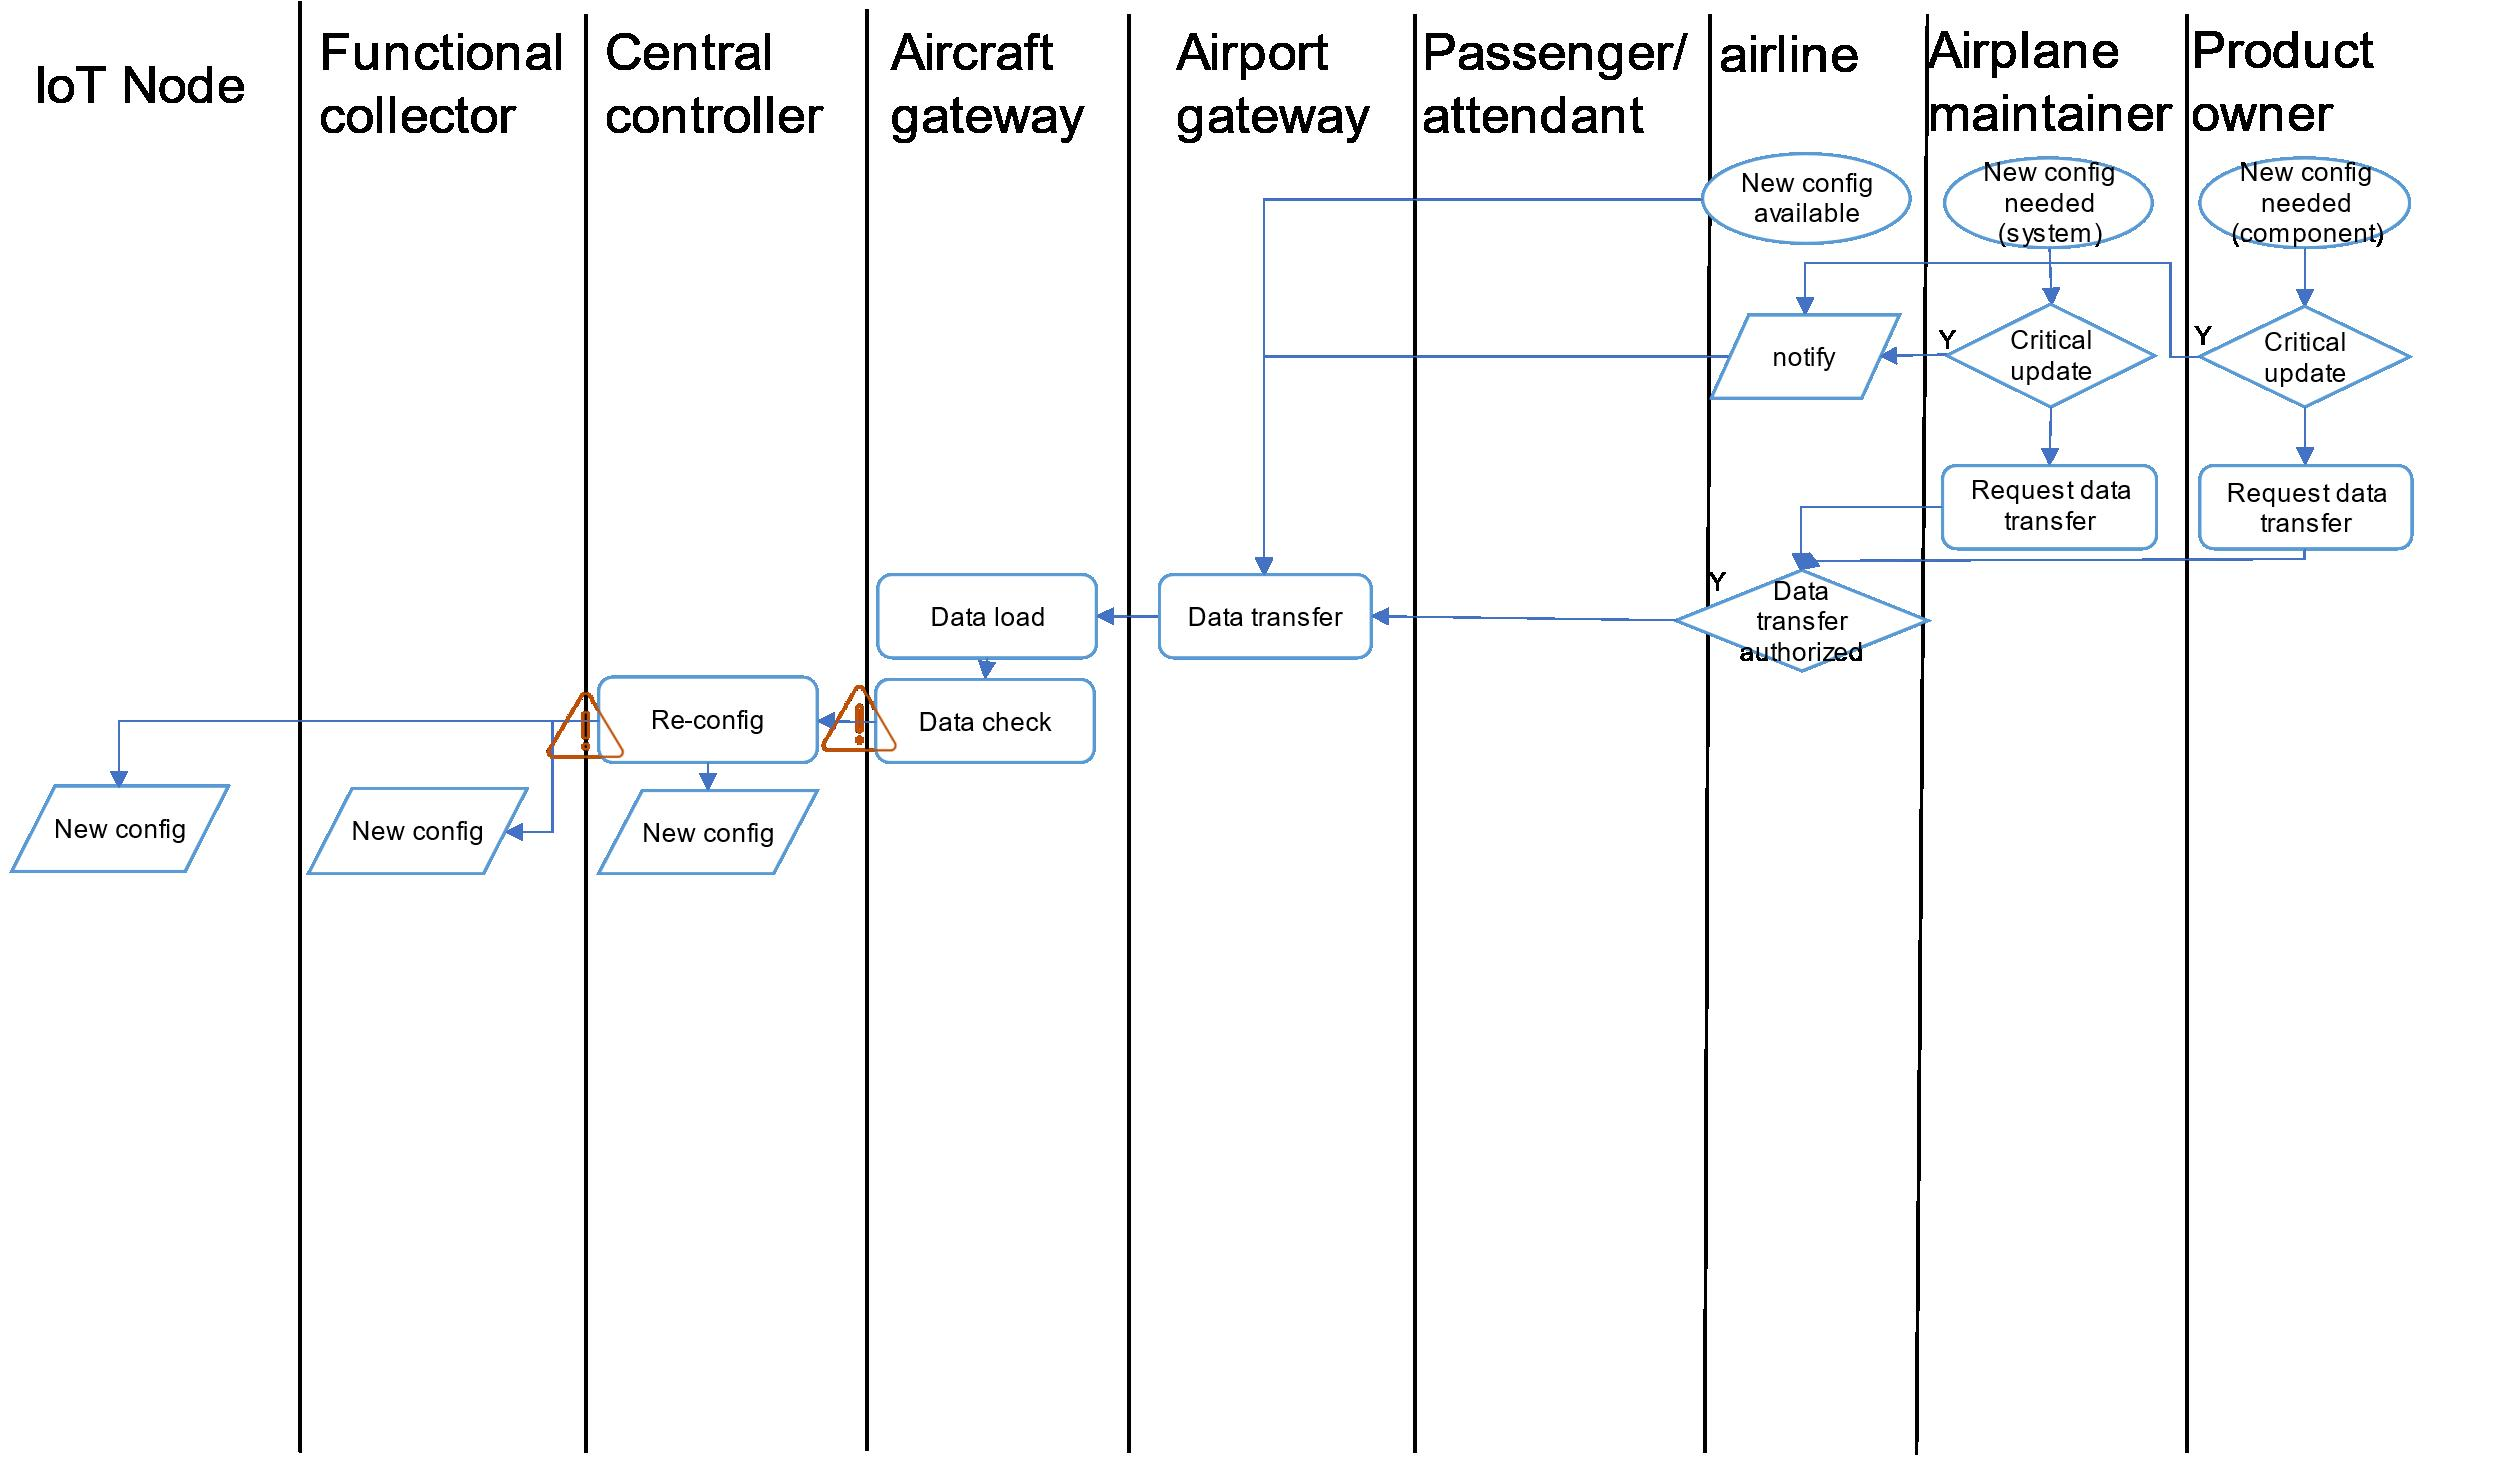
\includegraphics[width=0.95\textwidth]{figures/collins-s2-data-load-remote-config.jpg}
	\end{center}
	\caption{Collins Scenario 2.3: Data Load and Remote Reconfiguration}
	\label{fig:collins-s2-data-load-remote-config}
\end{figure}

\subsubsection{Post-Conditions}

After any of the sub-scenarios from Figures \ref{fig:collins-s2-data-collection-reconfig},
\ref{fig:collins-s2-data-unload-remote-analysis}, \ref{fig:collins-s2-data-load-remote-config}, the following
post-conditioned need to be met:

\begin{itemize}
	\item A new configuration, computed either locally or through the remote connection with the operations center
	      is available.
	\item Data from the aircraft are available for further analysis of Airline, Maintainer or Product Owner.
	\item For the configurations, integrity is verified, and confidentiality has been preserved (as it could
	      involve IP issues) in the process.
	\item For the data, in addition to integrity and confidentiality, it is important to also ensure availability
	      (to detect early sings of potential problems).

\end{itemize}

\subsubsection{Attack Scenario}

As an alternative flow of events, where an attack might happen, the main entry point is through the WiFi access point.
A rogue device could inject false data, configurations or software to facilitate subsequent attacks or even cause system
unavailability or device malfunctioning.
Alternatively in stealth mode, sensitive information could be captures and could be used to perpetrate other attacks.

% subsection System Operation and Monitoring (end

\subsection{LRU Replacement and Repurposing} % (fold)
\label{sub:LRU Replacement and Repurposing}

Akin to Scenario 1 in Subsection \ref{sub:Installation of Connected Cabin Systems} in this Scenario we also consider
similar steps to replace existing devices, with the difference, that the devices that replace the broken devices were
not exactly meant for this situation.

\begin{table}
	\caption{Actors involved}
	\label{tab:Actors involved lru}
	\begin{center}
		\begin{tabular}{ |p{2.5cm}|p{2.5cm}|p{2.5cm}|p{2.5cm}|p{2.5cm}| }
			\hline
			Airline & Airplane Maintainer & Product Owner & Maintenance Operator & Passenger, Attendant, Pilot \\
			\hline
			X       & X                   & X             & X                    & -                           \\
			\hline
		\end{tabular}
	\end{center}
\end{table}

\begin{table}
	\caption{Lifecycle stages involved}
	\label{tab:Lifecycle stages involved lru}
	\begin{center}
		\begin{tabular}{ |c|c|c|c|c| }
			\hline
			Bootstrapping & Operation & Update & Repurposing & Decommissioning \\
			\hline
			-             & -         & X      & X           & X               \\
			\hline
		\end{tabular}
	\end{center}
\end{table}

\subsubsection{Goals}

The goal of this scenario is to quickly replace a malfunctioning Central or Functional Controller, but a LRU is not
directly available. To minimize downtime, a spare LRU is retrieved from the same manufacturer and repurposed to the
specific target system. Airline, Airplane Maintainer, Product Owner, and Maintenance Operator are all involved to take
care of different steps in the process.

\subsubsection{Pre-Conditions}

Following pre-conditions must be met:

\begin{itemize}
	\item Actors involved can establish remote secure connection with aircraft.
	\item Airport has a spare LRU, that is compatible with CCS.
	\item The Maintenance Operator is provided access to the airplane and to the maintenance ports.
\end{itemize}

\subsubsection{Flow of Events}
\begin{figure}
	\begin{center}
		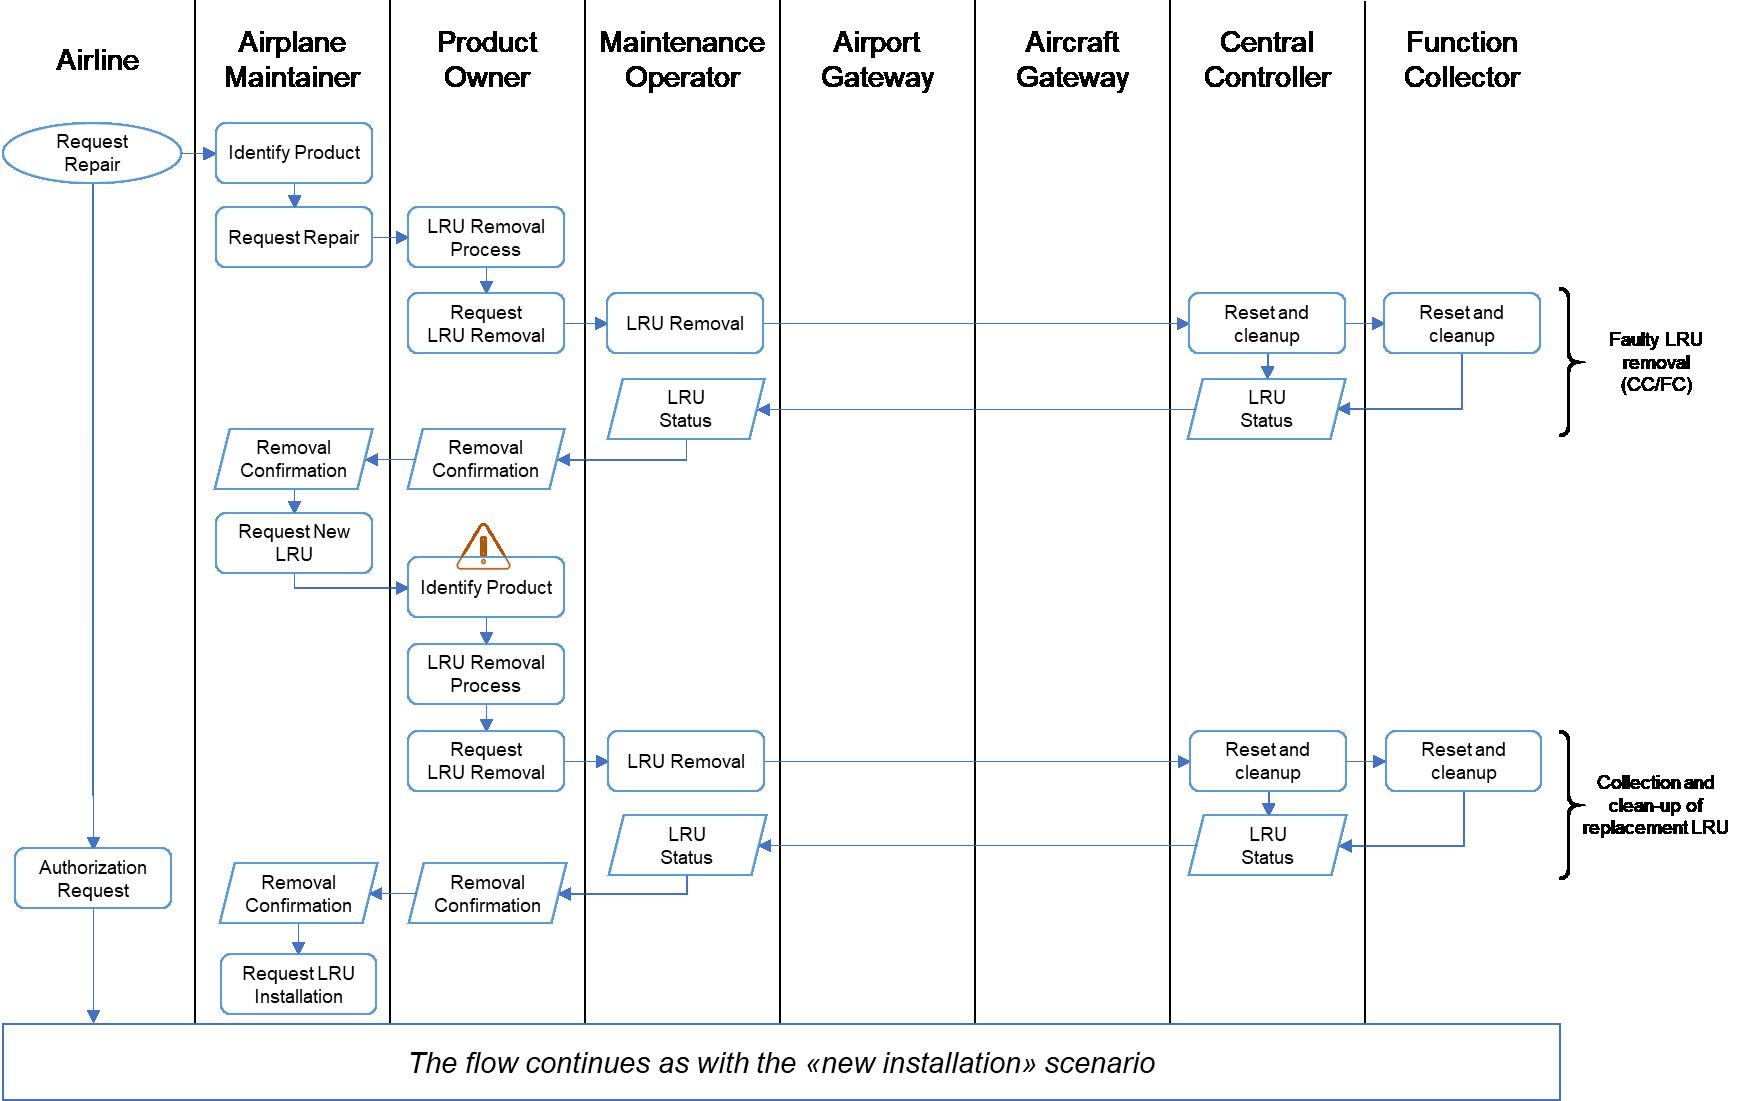
\includegraphics[width=0.95\textwidth]{figures/collins-s3-lru.jpg}
	\end{center}
	\caption{Collins Scenario 3: LRU Replacement}
	\label{fig:collins-s3-lru}
\end{figure}

\begin{itemize}
	\item The Airline requests to the Airplane Maintainer the repair of a cabin system, issuing and authorization
	      request to the Airport/Airplane gateways for following remote software update operations.
	\item The Airplane Maintainer identifies the target product, including its location, and the failure condition
	      then requests repair to Product Owner.
	\item The Product Owner starts the removal process of the LRU, including reset and cleanup
	\item Failed LRU removal executed locally by Maintenance Operator (also in charge of reset and cleanup)
	\item Product owner informs Airplane Maintainer of the removal and receives information of available replacement
	      LRUs.
	\item The replacement LRU shall be available from a remote location.
	\item The remaining flow proceeds as in Scenario 1 in Subsection \ref{sub:Installation of Connected Cabin Systems}

\end{itemize}

\subsubsection{Post-Conditions}
\begin{itemize}
	\item A new LRU  is deployed, integrated into network, updated with latest security patches and configured by
	      the Airline for specific needs
	\item CCS is registered with unique identifier and certificates are dispatched for authentication.
	\item For the configuration, integrity is verified and confidentiality has been preserved (for IP protection)
	      in the process
\end{itemize}

\subsubsection{Attack Scenario}

Attacks follow same pattern as in Subsection \ref{sub:Installation of Connected Cabin Systems} from Scenario 1.
An attacker can inject malicious software or a counterfeit LRU through the supply chain.
% subsection LRU Replacement and Repurposing (end)

\begin{figure}
	\begin{center}
		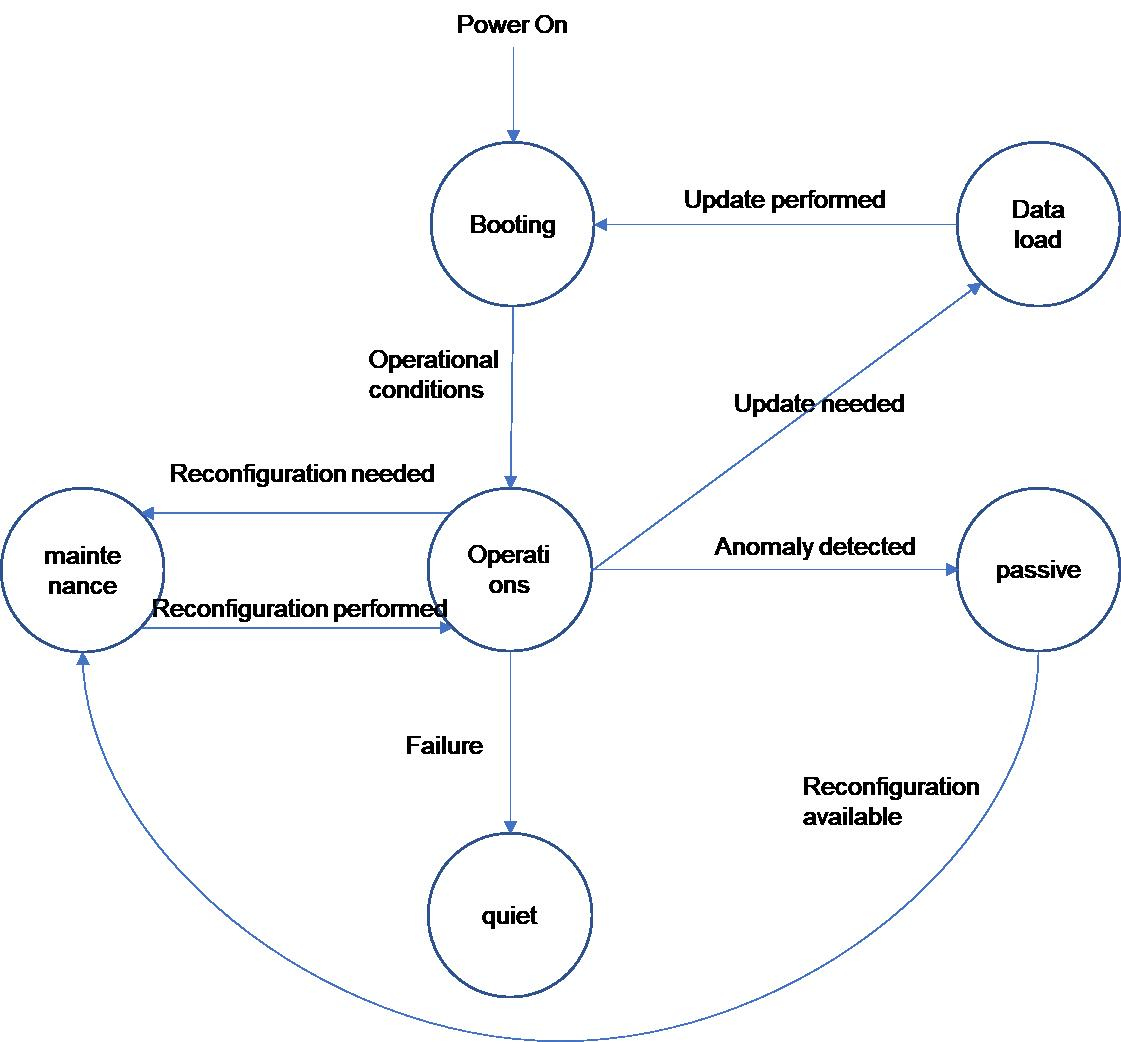
\includegraphics[width=0.95\textwidth]{figures/collins-opmodes.jpg}
	\end{center}
	\caption{Collins Operation Modes for an On-Board Device}
	\label{fig:collins-opmodes}
\end{figure}

% section Scenarios (end)

\section{Cybersecurity Assessment} % (fold)
\label{sec:Cybersecurity Assessment}

\begin{figure}
	\begin{center}
		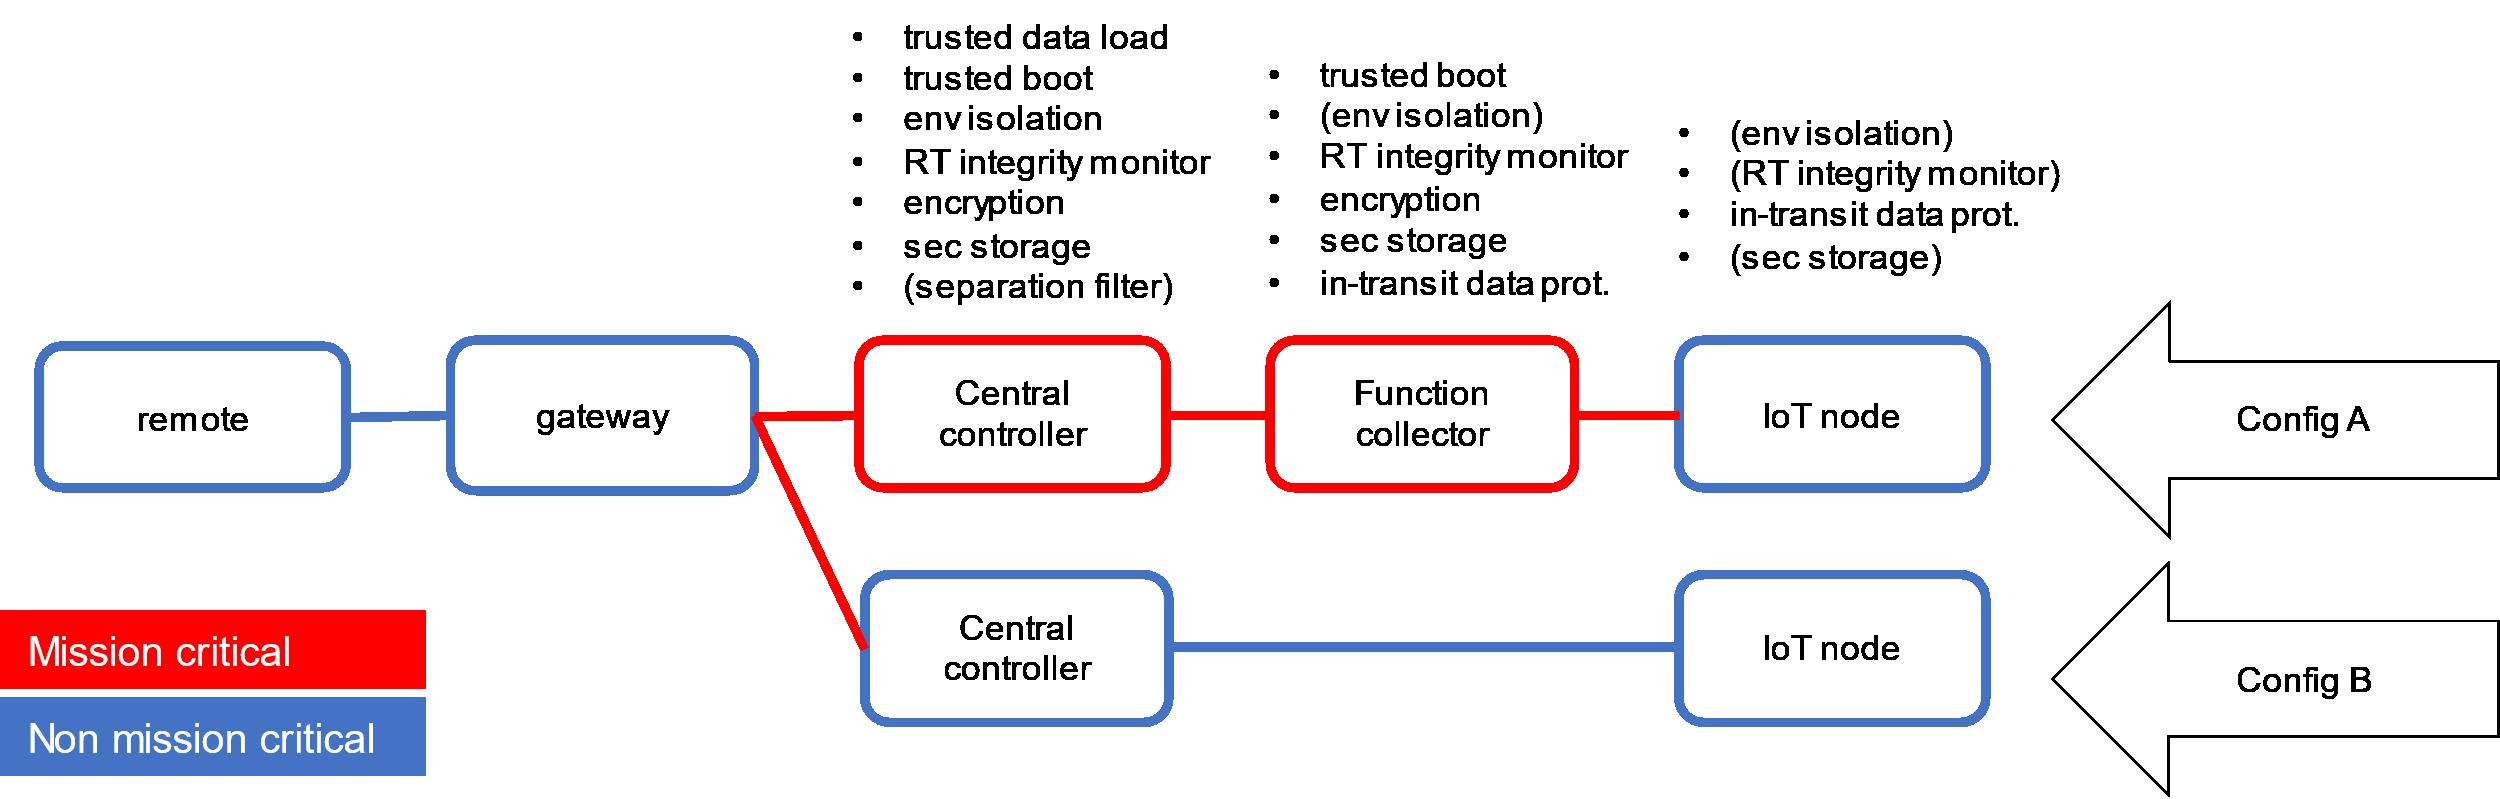
\includegraphics[width=0.95\textwidth]{figures/collins-sec-feat.jpg}
	\end{center}
	\caption{Collins Desired Security Features for the Different CCS Components}
	\label{fig:collins-sec-feat}
\end{figure}

The CERTIFY \cite{certifyproject2023} project describes following security levels:

\begin{itemize}
	\item Basic: Focus on common and simple cyber threats. User authentication, access controls and basic security
	      configuration.
	\item Substantial: More robust security measures including intrusion detection systems, IDS, incident response
	      plans and periodic security assessment.
	\item High: Requires organizations to establish comprehensive and proactive cybersecurity programs. Further
	      advanced security measures, network segmentation, encryption, continuous monitoring and regular
	      vulnerability assessments are needed. Threat intelligence sharing and regular security audits are also in
	      order.
\end{itemize}

Our use case, CCS, falls into the category of level \textit{HIGH}, as from a cybersecurity viewpoint the aircraft cabin
is considered a highly volatile and highly targeted environment.

% section Cybersecurity Assessment (end)

\chapter{Implementation}
% Explain the implementation specifics and elaborate on some architectural decisions made in 4

For our implementation it was important that we do not reinvent the wheel at each corner.

Choosing a DLT platform was not easy, as there were many options for Blockchains/DLTs but very few that were more or
less directly applicable to our thesis, which is IoTeX but its permissionless nature is not of good to us, as we would
like our network to be permissioned, which is another increase in security.

\chapter{Evaluation}


\chapter{Summary and Conclusions}



% Instead of manually listing the references, use bibtex to cite
% \begin{thebibliography}{99}
\addcontentsline{toc}{chapter}{Bibliography}

\bibitem{label} Autoren: Titel, Verlag, \url{http://...}, Datum.

\end{thebibliography}


\bibliographystyle{IEEEtran}
\bibliography{references}
\addcontentsline{toc}{chapter}{Bibliography}

\chapter*{Abbreviations}
\addcontentsline{toc}{chapter}{Abbreviations}
\markboth{ABBREVIATONS}{}

\abr{AAA}{Authentication, Authorization, and Accounting}
\abr{ACL}{Access Control List}
\abr{CCS}{Connected Cabin System}
\abr{CTIS}{Cyber Threat Information Sharing}
\abr{EVM}{Ethereum Virtual Machine}
\abr{GDPR}{General Data Protection Regulation}
\abr{HMI}{Human Machine Interface}
\abr{IDS}{Intrusion Detection System}
\abr{IFE}{In-flight Entertainment System}
\abr{IPS}{Intrusion Prevention System}
\abr{IoT}{Internet of Things}
\abr{LRU}{Line Replacable Unit}
\abr{MUD}{Manufacturer Usage Description}
\abr{NIST}{National Institute of Standards and Technology}
\abr{PHM}{Prognostics and Health Management}
\abr{PUF}{Physically Unclonable Function}
\abr{SCADA}{Supervisory control and data acquisition}
\abr{SRAM}{Static Random-Access Memory}
\abr{TEE}{Trusted Execution Environment}
\abr{TOE}{Target of Evaluation}
\abr{VC}{Verifiable Credential}

\chapter*{Glossary}
\addcontentsline{toc}{chapter}{Glossary}
\markboth{GLOSSARY}{}

% TODO: (aver) Ask Eryk if good as is
% https://csrc.nist.gov/glossary

\begin{description}
	\item[Authentication] Verifying the identity of a user, process, or device, often as a prerequisite to
		allowing access to resources in an information system. \cite{nist:glossary}
	\item[Accounting] Access privileges granted to a user, program, or process or the act of granting those
		privileges. \cite{nist:glossary}
	\item[Authorization] Authorization is the decision whether an entity is allowed to perform a particular action
		or not, e.g. whether a user is allowed to attach to a network or not.
	\item[Trust Model] In the trust model the issuer issues credential to a holder while the holder can prove
		identity by showing the credential to a verifier.
	\item [Manufacturer Usage Description] A component-based architecture specified in Request for Comments (RFC)
	      8520 that is designed to provide a means for end devices to signal to the network what sort of access and
	      network functionality they require to properly function. \cite{nist:glossary}
	\item [Cloud Computing] Cloud computing is the on-demand availability of computer system resources, especially
	      data storage and computing power, without direct active management by the user. \cite{nist:glossary}
	\item [Fog Computing] As an extension of Cloud computing, Fog Computing brings the computation closer to IoT
	      Edge devices. \cite{nist:glossary}
	\item [Edge Computing] Edge computing is the placement of storage and computing resources closer to source, where
	      the data is generated. \cite{nist:glossary}
	\item [Line-Replaceable Unit] modular component of airplane, designed to be replaced quickly
	\item [Firmware] Computer programs and data stored in hardware - typically in read-only memory (ROM) or
	      programmable read-only memory (PROM) - such that the programs and data cannot be dynamically written
	      or modified during execution of the programs. \cite{nist:glossary}
	\item [Trusted Execution Zone] An area or enclave protected by a system processor. \cite{nist:glossary}
\end{description}


\addcontentsline{toc}{chapter}{List of Figures}
\listoffigures
\addcontentsline{toc}{chapter}{List of Tables}
\listoftables
\addcontentsline{toc}{chapter}{List of Code Snippets and Examples}
\listoflistings

\appendix

\chapter{Installation Guidelines}

% \chapter{Contents of the CD}

\chapter{Code Snippets and Examples}

\begin{minted}{json}
{
  "ietf-mud:mud": {
    "mud-version": 1,
    "mud-url": "https://iot-device.example.com/dnsname",
    "last-update": "2019-01-15T10:22:47+00:00",
    "cache-validity": 48,
    "is-supported": true,
    "systeminfo": "This is an example of a device that just wants to talk
		    to its cloud service",
    "mfg-name": "Example, Inc.",
    "documentation": "https://iot-device.example.com/doc/dnsname",
    "model-name": "dnsname",
    "from-device-policy": {
      "access-lists": {
        "access-list": [
          {
            "name": "mud-96898-v4fr"
          },
          {
            "name": "mud-96898-v6fr"
          }
        ]
      }
    },
    "to-device-policy": {
      "access-lists": {
        "access-list": [
          {
            "name": "mud-96898-v4to"
          },
          {
            "name": "mud-96898-v6to"
          }
        ]
      }
    }
  },
  "ietf-access-control-list:acls": {
    "acl": [
      {
        "name": "mud-96898-v4to",
        "type": "ipv4-acl-type",
        "aces": {
          "ace": [
            {
              "name": "cl0-todev",
              "matches": {
                "ipv4": {
                  "ietf-acldns:src-dnsname": "cloud-service.example.com"
                }
              },
              "actions": {
                "forwarding": "accept"
              }
            }
          ]
        }
      },
      {
        "name": "mud-96898-v4fr",
        "type": "ipv4-acl-type",
        "aces": {
          "ace": [
            {
              "name": "cl0-frdev",
              "matches": {
                "ipv4": {
                  "ietf-acldns:dst-dnsname": "cloud-service.example.com"
                }
              },
              "actions": {
                "forwarding": "accept"
              }
            }
          ]
        }
      },
      {
        "name": "mud-96898-v6to",
        "type": "ipv6-acl-type",
        "aces": {
          "ace": [
            {
              "name": "cl0-todev",
              "matches": {
                "ipv6": {
                  "ietf-acldns:src-dnsname": "cloud-service.example.com"
                }
              },
              "actions": {
                "forwarding": "accept"
              }
            }
          ]
        }
      },
      {
        "name": "mud-96898-v6fr",
        "type": "ipv6-acl-type",
        "aces": {
          "ace": [
            {
              "name": "cl0-frdev",
              "matches": {
                "ipv6": {
                  "ietf-acldns:dst-dnsname": "cloud-service.example.com"
                }
              },
              "actions": {
                "forwarding": "accept"
              }
            }
          ]
        }
      }
    ]
  }
}
\end{minted}
% TODO: (aver) add source
\captionof{listing}{Example MUD file \cite{mudexample}}
\label{code:mud}


\end{document}
